%----------------------------------------------------------------------------------------
%	PACKAGES AND OTHER DOCUMENT CONFIGURATIONS
%----------------------------------------------------------------------------------------

\documentclass[
12pt, % The default document font size, options: 10pt, 11pt, 12pt
%oneside, % Two side (alternating margins) for binding by default, uncomment to switch to one side
english, % ngerman for German
singlespacing, % Single line spacing, alternatives: singlespacing, onehalfspacing or doublespacing
%draft, % Uncomment to enable draft mode (no pictures, no links, overfull hboxes indicated)
%nolistspacing, % If the document is onehalfspacing or doublespacing, uncomment this to set spacing in lists to single
%liststotoc, % Uncomment to add the list of figures/tables/etc to the table of contents
%toctotoc, % Uncomment to add the main table of contents to the table of contents
%parskip, % Uncomment to add space between paragraphs
%nohyperref, % Uncomment to not load the hyperref package
headsepline, % Uncomment to get a line under the header
%chapterinoneline, % Uncomment to place the chapter title next to the number on one line
%consistentlayout, % Uncomment to change the layout of the declaration, abstract and acknowledgements pages to match the default layout
]{MasterThesis} % The class file specifying the document structure

%%% Added a few more style commands to ensure spacing
\usepackage{blindtext}
\setlength{\parskip}{\baselineskip}
\setlength{\parindent}{0pt}
\AtBeginDocument{\addtocontents{toc}{\protect\setlength{\parskip}{0pt}}}
\AtBeginDocument{\addtocontents{lof}{\protect\setlength{\parskip}{0pt}}}
%%%

\usepackage[utf8]{inputenc} % Required for inputting international  characters
\usepackage[T1]{fontenc} % Output font encoding for international characters

\usepackage{mathpazo} % Use the Palatino font by default

\usepackage[backend=biber,style=numeric,natbib=true]{biblatex} % Use the bibtex backend with the authoryear citation style (which resembles APA)

\addbibresource{References.bib} % The filename of the bibliography

\usepackage[autostyle=true]{csquotes} % Required to generate language-dependent quotes in the bibliography

%----------------------------------------------------------------------------------------
%	MARGIN SETTINGS
%----------------------------------------------------------------------------------------

\geometry{
	paper=a4paper, % Change to letterpaper for US letter
	inner=2.5cm, % Inner margin
	outer=2.8cm, % Outer margin
	bindingoffset=.5cm, % Binding offset
	top=1.5cm, % Top margin
	bottom=1.5cm, % Bottom margin
	%showframe, % Uncomment to show how the type block is set on the page
}

%   Self-defined commands
%   Text coloring commands

%   include own packages
\usepackage{amssymb, amsfonts, amsmath, amsthm}
\usepackage{float}
\usepackage[font=footnotesize, labelfont=bf, justification=justified, format=plain]{caption} % 'format=plain' avoids hanging indentation

%   Own commands
\usepackage{mydraft}
\usepackage{mysty}

\theoremstyle{plain}
\newtheorem{theorem}{Theorem}[chapter]
\newtheorem{corollary}[theorem]{Corollary}
\newtheorem{lemma}[theorem]{Lemma}
  
%\theoremstyle{definition}
\newtheorem{proposition}[theorem]{Proposition}
\newtheorem{definition}[theorem]{Definition}
\newtheorem{example}[theorem]{Example}
\newtheorem{conjecture}[theorem]{Conjecture}

\theoremstyle{remark}
\newtheorem{remark}[theorem]{Remark}

\setlist[itemize]{topsep=0pt}

\captionsetup[table]{labelsep=space}
\captionsetup[figure]{labelsep=space}

% Category theory notation
%\newcommand{\cat}{%
%\mathbf%
%}
%\newcommand{\domain}[1]{%
%    mathrm{dom}(#1)%
%}
%\newcommand{\codomain}[1]{%
%    \mathrm{cod}(#1)%
%}
%\newcommand{\idarrow}[1][]{%
%    \mathbf{1}_{#1}%
%}

%	THESIS INFORMATION
%----------------------------------------------------------------------------------------
%	THESIS INFORMATION
%----------------------------------------------------------------------------------------

\thesistitle{A Non-Sculpting Theorem in Non-Interleaving Models for Concurrency} % Your thesis title, this is used in the title and abstract, print it elsewhere with \ttitle
\supervisor{\textbf{Christian Johansen}, \univname} % Your supervisor's name, this is used in the title page, print it elsewhere with \supname
\cosupervisor{\textbf{Ulrich Fahrenberg}, Ecole Polytechnique, France} % Your co-supervisor's name, this is used in the title page, print it elsewhere with \csupname
\ccosupervisor{\textbf{Martin Steffen}, \univname} % Your co-supervisor's name, this is used in the title page, print it elsewhere with \ccsupname
\cccosupervisor{\textbf{Olaf Owe}, \univname} % Your co-supervisor's name, this is used in the title page, print it elsewhere with \cccsupname
\examiner{} % Your examiner's name, this is not currently used anywhere in the template, print it elsewhere with \examname
\degree{Master of Science (MSc)} % Your degree name, this is used in the title page and abstract, print it elsewhere with \degreename
\author{Christopher A. Trotter} % Your name, this is used in the title page and abstract, print it elsewhere with \authorname
\addresses{} % Your address, this is not currently used anywhere in the template, print it elsewhere with \addressname

\subject{Theoretical Computer Science} % Your subject area, this is not currently used anywhere in the template, print it elsewhere with \subjectname
\keywords{concurrency, algebraic topology, category theory} % Keywords for your thesis, this is not currently used anywhere in the template, print it elsewhere with \keywordnames
\university{\href{http://www.uio.no}{University of Oslo}} % Your university's name and URL, this is used in the title page and abstract, print it elsewhere with \univname
\department{\href{http://www.uio.ifi.no}{Department of Informatics}} % Your department's name and URL, this is used in the title page and abstract, print it elsewhere with \deptname
\group{\href{https://www.mn.uio.no/ifi/english/research/groups/psy/}{Reliable Systems (PSY)}} % Your research group's name and URL, this is used in the title page, print it elsewhere with \groupname
\faculty{\href{http://www.mn.uio.no/english/}{The Faculty of Mathematics and Natural Sciences}} % Your faculty's name and URL, this is used in the title page and abstract, print it elsewhere with \facname

\AtBeginDocument{
\hypersetup{pdftitle=\ttitle} % Set the PDF's title to your title
\hypersetup{pdfauthor=\authorname} % Set the PDF's author to your name
\hypersetup{pdfkeywords=\keywordnames} % Set the PDF's keywords to your keywords
}

%   Abbreviations/acronyms list
\usepackage[toc,acronym]{glossaries}

%   UiO master thesis front page
\usepackage{ifimasterforside}

%   Title of master thesis
\title{A Non-Sculpting Theorem in Non-Interleaving Models for Concurrency}

\usepackage{etoolbox}
\patchcmd{\thebibliography}{\section}{\section}{}{}

%   Making acronyms
%\makeglossaries

\begin{document}

%\ififorside

%	TITLE PAGE
%----------------------------------------------------------------------------------------
%	TITLE PAGE
%----------------------------------------------------------------------------------------

\begin{titlepage}
\begin{center}

%\vspace*{.06\textheight}
%{\scshape\LARGE \univname\par}\vspace{1.5cm} % University name
%\textsc{\Large Master Thesis}\\[0.5cm] % Thesis type

%\HRule \\[0.4cm] % Horizontal line
{\huge \bfseries \ttitle\par}\vspace{1cm} % Thesis title
%\HRule \\[1.5cm] % Horizontal line

%\vfill

\Large \textit{Thesis submitted in partial fulfillment of the requirements for the degree of\\}
\textit{\textbf{\degreename}}\\ % University requirement text
\textit{to the \facname,}\\
\textit{at the \univname.}\\[1cm]

\LARGE \textbf{\authorname}\\
\Large \textit{\groupname\\\deptname, \univname}\\[1cm] % Research group name and department name


\includegraphics[scale=0.5]{Pictures/uioLogo.jpg}\\[1cm]

\Large \textit{Supervisors:}\\
\href{http://folk.uio.no/cristi/master_topics_prisacariu.php}{\supname} \\ % Supervisor name - remove the \href bracket to remove the link
\href{http://www.lix.polytechnique.fr/Labo/Ulrich.Fahrenberg/}{\csupname} \\ % Supervisor name - remove the \href bracket to remove the link
\href{http://heim.ifi.uio.no/~msteffen/}{\ccsupname} \\ % Supervisor name - remove the \href bracket to remove the link
\href{http://olaf.at.ifi.uio.no/}{\cccsupname} % Supervisor name - remove the \href bracket to remove the link


\vfill

{\large \today}\\[4cm] % Date
%\includegraphics{Logo} % University/department logo - uncomment to place it
 
\vfill
\end{center}
\end{titlepage}

\frontmatter % Use roman page numbering style (i, ii, iii, iv...) for the pre-content pages

\pagestyle{plain} % Default to the plain heading style until the thesis style is called for the body content

%	ABSTRACT PAGE
%\addchap*{Abstract}
%----------------------------------------------------------------------------------------
%	ABSTRACT PAGE
%----------------------------------------------------------------------------------------

\chapter*{Abstract}
\addchaptertocentry{\abstractname} % Add the abstract to the table of contents
    
    The geometric model, Higher-dimensional automata (HDA), is a useful and general model for non-interleaving concurrency. In a non-interleaving approach to concurrency, more than one event may happen concurrently and one differentiates between concurrent and interleaving executions, satisfying $a \parallel b \neq a.b + b.a$. HDA also encompass all other commonly used models of concurrency. However, due to generality HDAs are challenging to work with. Vaughan Pratt introduced sculptures and Chu spaces as models which retain some of the good properties of HDA as well as being easier to work with. Recently, Johansen has introduced ST-structures as another event-based formalism for the same purpose.
    
    This thesis gives a precise definition of sculptures, following the intuition of Pratt, where one can think of the process of modelling a concurrent system using higher-dimensional automata as a \emph{sculpting} process as follows. Take one single higher-dimensional cube, having enough concurrency, and remove cells until the desired concurrent behaviour is obtained. This is different from \emph{composition} where a system is built by composing together smaller systems, which in higher-dimensional automata is done by gluing together cubes.
    
    We also develop an algorithm to decide whether a higher-dimensional automaton is a sculpture or not, and use this to show that some simple acyclic higher-dimensional automata are not sculptures. We believe that this contradicts Pratt's intuition that sculptures suffice for the modelling of concurrent behaviour, because not all higher-dimensional automata can be sculpted.
    
    We show that sculptures, Chu spaces and ST-structures are in close correspondence. This nicely captures Pratt's event-state duality and tightens the correlation between ST-structures and higher-dimensional automata, which was left as an open problem by Johansen.

%	ACKNOWLEDGEMENTS
%----------------------------------------------------------------------------------------
%	ACKNOWLEDGEMENTS
%----------------------------------------------------------------------------------------

\chapter*{Acknowledgements}
\addchaptertocentry{\acknowledgementname} % Add the acknowledgements to the table of contents

\emph{A significant portion of this thesis represents joint work with my supervisors Christian Johansen and Ulrich Fahrenberg. They have been instrumental in shaping my ideas of concurrent systems and my view of research in general, and their support and intellectual guidance have made this thesis possible. I am also indebted to my other supervisors, Martin Steffen and Olaf Owe. Thank you for sharing your knowledge, offering advice, and for every one of our helpful discussions.}

\emph{So many others have also offered their help along the way. Among them I would like to thank my brother James for taking the time to listen and for offering his valuable insight and perspective. I would also like to thank Bibek Kabi for all the coffee breaks with insightful conversations while I was in Paris as part of my internship. I am grateful to my fellow students who have never turned me down when I have asked questions. In particular, I want to mention Marius Andresen, Mateusz Zych, Norah Nguyen and Ratan Thapa.}

\emph{I would like to thank my family and friends who have supported me along the way. Thank you so much.}

\emph{Last, but certainly not least. Thank you, Zahra.}

\null\hfill \emph{Christopher A. Trotter,}\\
\null\hfill \emph{November 2018}

%	LIST OF CONTENTS/FIGURES/TABLES PAGES
%----------------------------------------------------------------------------------------
%	LIST OF CONTENTS/FIGURES/TABLES PAGES
%----------------------------------------------------------------------------------------

\tableofcontents % Prints the main table of contents

\listoffigures % Prints the list of figures

%\listoftables % Prints the list of tables

%----------------------------------------------------------------------------------------
%	THESIS CONTENT - CHAPTERS
%----------------------------------------------------------------------------------------

\mainmatter % Begin numeric (1,2,3...) page numbering

\pagestyle{thesis} % Return the page headers back to the "thesis" style

% Include the chapters of the thesis as separate files from the Chapters folder
% Uncomment the lines as you write the chapters
In this chapter we present non-interleaving models of concurrency that generalize the independence of two, or more, events. We present a geometric model of concurrency which is an algebraic structure able to capture the main characteristic of \emph{both} interleaving and non-interleaving models. We show both a state-based model, higher-dimensional automata, and an event-based model, ST-structures, capable of distinguishing an arbitrary number of events. Also, we present Chu spaces as a model able to present state-based and event-based models symmetrically, such that there is a way to present the event-state duality symmetrically. 

The models mentioned so far have been based on interleaving computation steps to capture all the possible behaviours of a concurrent system. Recall the interleaving square, in Figure \ref{fig:transition-system}, where we have four states $s_{1}$, $s_{2}$, $s_{3}$ and $s_{4}$ and four transitions, where two of the transitions are labeled $a$ and the other two transitions are labeled $b$. We see that these two actions $a$ and $b$ can be executed in either order, ending in the same state each way, such that $a$ and $b$ are mutually exclusive. By design, interleaving models depend on the notion of \emph{atomic} actions, that is, actions that are indivisible.

The assumption of atomic actions is reasonable for events that are mutually exclusive, meaning they cannot occur simultaneously. For example, a vending machine able to provide a single item at a time, like a snack or a beverage. If we want two items, such as a chocolate and a beverage, from the vending machine, then either the chocolate will be released followed by the beverage or first the beverage followed by the chocolate. However, for events that are truly independent, such as a vending machine able to provide two, or more, items at a time, then their order of occurrence would be rendered irrelevant $-$ two items would be released at the same time from the vending machine. Models that only allow interleaving are unable to distinguish these two vending machine. Instead, we will consider the non-interleaving models of concurrency, such as \emph{asynchronous transition systems} \cite{winskel95modelsCategory} and \emph{higher-dimensional automata} \cite{pratt91hda}, \emph{ST-structures} \cite{Johansen16STstruct} and \emph{Chu spaces} \cite{gupta94phd_Chu}, which are able to distinguishing between these two vending machines. Thus, we allow receiving multiple items after each other, or all at the same time. Going further, we may even have a combination of the alternatives.

For didactic and historical reasons, we will review asynchronous transition systems where we introduce an independence relation between the occurrence of events. The independence relation is able to express the mutual exclusion and non-interleaving of two events. Asynchronous transition systems may be considered a bridge between transition systems, used up until now, and the higher-dimensional automata, introduced in Section \ref{sec:higher-dimensional-automata}. Higher-dimensional automata are expressive and can encode the independence of an arbitrary number of events, rather than only pairs of events.

Higher-dimensional automata are \emph{algebraic structures} which can be interpreted geometrically, roughly as topological spaces with a sense of direction to incorporate a notion of irreversible time. A topological space with a sense of direction makes it possible to determine the order of an execution. Intuitively, a higher-dimensional automaton is an automaton with nicely incorporated squares, cubes and higher-dimensional cubes, which represent the independence of events. A main characteristic of higher-dimensional automata is to be able to capture what happens \emph{during} an execution. ST-structure is the event-based counterpart of higher-dimensional automata which is able to precisely identify events, and also capture what happens during an execution. As shown by Johansen in \cite{Johansen16STstruct}, higher-dimensional automata cannot precisely identify events. For example, the asymmetric conflict shown in \cite[Figure 5]{Johansen16STstruct} and presented in Section \ref{sec:st-structure-and-hda}. However, we may faithfully represent the asymmetric conflict as a ST-structure.
\section{The contributions of this thesis}
    Part of this thesis is dedicated to giving an introduction to concurrency models, where we focus on non-interleaving models of concurrency capable of capturing the independence of arbitrary number of events. In order to achieve this, we have included a review of several existing models of concurrency in Chapter \ref{chap:traditional-models-for-concurrency} and \ref{chap:An introduction to models for true concurrency}, including transition systems, event structures, configuration structures, asynchronous transition systems, higher dimensional automata, ST-structure and Chu spaces. This part does not represent new work in itself, and the relationships between the models in Chapter \ref{chap:Relationship with other models of true concurrency} have been investigated and are known in the geometric models of concurrency literature.
    
    On the other hand, we show the ideas the above mentioned models of concurrency have contributed to understanding both higher-dimensional automata and sculptures. In Chapter \ref{chap:traditional-models-for-concurrency}, we expend some effort to explain the difference between interleaving and non-interleaving models, and the need for non-interleaving models to incrementally develop concurrent systems by action refinement. Also, we investigate the event-state duality of non-interleaving models  to better understanding the current research being done. Specifically, investigating event-state duality in higher-dimensional automata by ST-structures and Chu spaces.
    
    The main contribution is the method of sculpting that is presented in Chapter \ref{chap:sculpting-in-concurrency}. Sculpting is a method of modelling concurrent behaviour of higher-dimensional automata. We investigate a conjecture posed by Vaughan Pratt in \cite{Pratt00Sculptures}. The conjecture is whether any higher-dimensional automata can be obtained using the sculpting method. We first define precisely the sculpting method, following again the intuition of Pratt that sculpting is similar to subalgebras. We develop an algorithm to decide whether an higher-dimensional automaton can be sculpted or not, and show several simple examples of \emph{acyclic} higher-dimensional automata which are not sculptures.
    
    We attempt to precisely identify the class of higher-dimensional automata which by sculpting can identify events. From the work by Johansen \cite{Johansen16STstruct}, we known higher-dimensional automata are in general not good at identifying events. However, as we show in this thesis, sculptures are well suited to represent the events, thus overcoming the problem identified in \cite[Figure 5]{Johansen16STstruct}. For example, the asymmetric conflict cannot be represented as a higher-dimensional automata, but can be faithfully represented as a sculpture or as an ST-structure. Going further, sculptures are one response to the event-state duality of Pratt \cite{Pratt02eventStateDuality} in higher-dimensional automata.
    
   
\section{The organisation of this thesis}
In this section, we briefly present the organisation of the thesis with an overview of each chapter.

\textbf{Chapter 2} presents transition systems and event structures. Transition systems are interleaving models of concurrency and can be interpreted, geometrically, as one-dimensional spaces consisting of edges (its transitions) meeting and branching at vertices (its states). Transition systems provide the foundation to understand the generalization of the geometric model of concurrency. Also, transition systems are automata and considered one side of a duality, where schedules, or events, is the other. Event structures are schedules which provide the necessary background for understanding ST-structures and provide the intuition of the state-event duality presented in Chapter \ref{chap:Relationship with other models of true concurrency}. 

\textbf{Chapter 3} presents the non-interleaving models of concurrency, specifically, asynchronous transition systems, higher-dimensional automata, ST-structures and Chu spaces. We consider asynchronous transition systems to be the bridge between transition systems and higher-dimensional automata. Asynchronous transition systems are seen, geometrically, as a two-dimensional space extending the transition systems by considering surfaces (its independence relations) between edges (its transitions) and vertices (its states). Higher-dimensional automata are a generalization of both transition systems and asynchronous transition systems. We consider higher-dimensional automata as an $n$-dimensional space consisting of points, segments, squares, cubes, and higher-dimensional cubes. ST-structures are the event-based counterpart of higher-dimensional automata capable of capturing a main characteristic of higher-dimensional automata, that is, to be able to see what happens during a concurrent execution. Chu spaces are considered a response to the state-event duality problem and introduce the notion of "\emph{sculpting}", which we present in Chapter \ref{chap:sculpting-in-concurrency}.

\textbf{Chapter 4} presents the relationship between certain non-interleaving models of concurrency. Specifically, we will relate higher-dimensional automata and ST-structures as well as ST-structures and Chu spaces. Higher-dimensional automata are not good at identifying events as show in Example \ref{exp:asymmetric-conflict}, but can be faithfully interpreted as ST-structures to identify events. In Example \ref{exp:asymmetric-conflict}, isomorphic higher-dimensional automata are interpreted as non-isomorphic ST-structures. Hence, there is not an embedding, that is, an injective morphism, from $\allST$ to $\allHDA$. We also show in Figure \ref{fig:Unfolding-HDA} that non-isomorphic higher-dimensional automata interpreted as ST-structures become isomorphic ST-structures, meaning there is not an embedding from $\allHDA$ to $\allST$. Hence, higher-dimensional automata are neither more, or less, expressive than ST-structures. We investigate the relationship between Chu spaces and ST-structure to better understand the state-event duality.

\textbf{Chapter 5} presents the method "\emph{sculpting}" which has not been studied for higher-dimensional automata before. We investigate the relationship between sculptures and ST-structures to tighten the correlation between ST-structures and higher-dimensional automata, which was left open in \cite{Johansen16STstruct}. We develop an algorithm to decide whether an higher-dimensional automaton can be sculpted or not, and show several simple examples of acyclic higher-dimensional automata which are not sculptures. We believe that this contradicts Pratt's conjecture.

\textbf{Chapter 6} presents some concluding remarks, summarizes the contributions of the thesis and offers some ideas that can be pursued in future work.
\chapter{An introduction to traditional models of concurrency}
\label{chap:traditional-models-for-concurrency}

    For the most part, early models of computation, such as Turing Machines \cite{turing_1937}, are sequential, meaning that there is a strict order in which computational steps happen. The strict ordering ensures that the sequence of computational steps are unambiguous, such that one could provide a single history of the executed computation. For sequential computation, the $\lambda$-calculus has become a fundamental unifying formalism. This framework is also accommodated by a rich variety of developments such as types and higher-type computation, program logic, operational semantics, and denotational semantics. However, concurrent computation has yet to see a unifying framework in the way that $\lambda$-calculus is for sequential computation.
    
    There has been extensive research within the field of concurrency theory to approach a unifying concept, and an outline of many deep, fundamental results was done by Garavel in \cite{gravel08summary}. In this thesis, we will investigate one of the opportunities mentioned by Garavel and present the notion of sculpting for higher-dimensional automata, as a result. The opportunity described was the idea of having models everywhere and a way to transform one model into another. Specifically, models for different purposes and a way to translate between them. Considering this opportunity would unify several pre-existing concepts such as translation and refinement.

    Since the 1960s, a wide variety of models of concurrency have been proposed. One of the first proposals was Petri nets. During the past decades, there have been other proposals for models of concurrency, such as transition systems, higher dimensional automata and event structures. Even though the nature of these models are very different, they have shown to have a tight relation to each other, as presented by Winskel \cite{winskel95modelsCategory} and Goubault \cite{Goubault18RelationshipsModelsForConcurrency}. Because of this relation, we classify models of concurrency as state-based, \emph{automata}, or event-based models, \emph{schedules}. Also, we further classify these as interleaving or non-interleaving models. For sequential behaviour these classes are considered equivalent. In this thesis, we will  focus on the classification of interleaving versus non-interleaving models. We will first review \emph{transition systems} as an interleaving model and show how they fall short of our intuition of concurrent behaviour.
\section{Transition systems}
\label{sec:ordinary-transition-systems}
    Transition systems are well established semantic models for both sequential and concurrent systems. A transition system can be viewed as a directed graph, called a state transition graph, whose vertices are states and edges are transitions between states. We may consider a transition system, as shown in Figure \ref{fig:transition-system}, where we have four states $s_{1}$, $s_{2}$, $s_{3}$, and $s_{4}$, for example, representing a program changing a value of a variable at different times of its execution. We also have four transitions, two of which are labeled $a$ and another two which are labeled $b$. We can also have the same label $a$ for both events, giving rise to the notion of \emph{autoconcurrency}. These four transitions, represent two instructions of a program that change the state of the machine from the source of its arrow to its corresponding target. This is formalized by using a transition relation. We will refer to this transition system as the \emph{interleaving square}, similar to what has been done by Pratt \cite{Pratt00Sculptures} and van Glabbeek \cite{Glabbeek06HDA}. We will use the same notation and definitions as Winskel and Nielsen in \cite{winskel95modelsCategory}.
    
    \begin{figure}[ht]
        \centering
        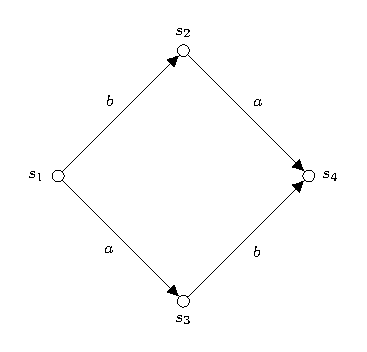
\includegraphics[scale=1.1]{Figures/2.Models-for-concurrency/transition-system.pdf}
        \captionof{figure}[A transition system.]{A transition system with four states, $s_{1}, s_{2}, s_{3}$, and $s_{4}$, and four transitions, two of which are labeled $a$ and the other two are labeled $b$. These four transitions present the interleaving of two instructions. The interleaving is namely the permutation of all possible executions of these two instructions. This transition system is called the interleaving square because of the way the interleaving of two instructions form a square.}
        \label{fig:transition-system}
      
    \end{figure}
    
    \begin{definition}[Transition system \cite{winskel95modelsCategory}]\label{def:transition-system}
        A transition system is a structure ($\mathcal{S}, i, \mathcal{L}, Tran$) where,
        \begin{itemize}
            \item $\mathcal{S}$ is a set of states with initial state i,
            \item $\mathcal{L}$ is a set of labels, and
            \item $Tran \subseteq \mathcal{S} \times \mathcal{L} \times \mathcal{S}$ is the transition relation
        \end{itemize}
    \end{definition}
    
    We will write $s \xrightarrow{a} s'$ to indicate  that $(s,a,s') \in Tran$.
    
    Morphisms between transition systems often describe the relationships between processes. These kind of relations are described by Winskel and Nielsen in \cite{winskel95modelsCategory}, where one process may be a component of another or perhaps one process may refine another process. By defining morphisms as simulations between transition systems, we are able to describe the relationship between processes. For example, a simulation is where a transition system $\mathcal{T}$ simulates a transition system $\mathcal{T}^{'}$, meaning that when $\mathcal{T}^{'}$ can execute some action $a$ then there must exists an $a$ in $\mathcal{T}$ that can be executed.
    
    \begin{definition}[Morphism of transition systems \cite{winskel95modelsCategory}]\label{def:morphism-of-transition-system}
        A morphism from one transition system, $\mathcal{T}$, to another, $\mathcal{T}^{'}$ , will be a pair $(\sigma, \lambda)$ in which
        \begin{itemize}
            \item $\sigma$ is a function from the states of $\mathcal{T}$ to those of $\mathcal{T}^{'}$ .
            \item $\lambda$ is a partial function from the labels of $\mathcal{T}$ to those of $\mathcal{T}^{'}$ such that for any transition $s \xrightarrow{a} s'$ of $\mathcal{T}$ if $\lambda(a)$ is defined, then $\sigma(s) \xrightarrow{\lambda(a)} \sigma(s')$ is a transition of $\mathcal{T}^{'}$ ; otherwise, if $\lambda(a)$ is undefined, then $\sigma(s) = \sigma(s')$.
        \end{itemize}
    \end{definition}
    
    In our notation, we have used $\mathcal{L}$ to stand for the set of labels for events, as well as to stand for the actual set of those events. However, sometimes it might be useful to make a distinction between the events themselves and to explicitly give a labeling as a function. For instance, this is important when treating \emph{relabeling} which leads to categorical fibrational situations \cite{winskel95modelsCategory}. To make the distinction between labels of events and the actual events clearer, we will replace $\mathcal{L}$ with $E$ and refer to its elements as \emph{events}.
    
    \begin{definition}[Labeled transition system \cite{winskel95modelsCategory}]\label{def:labeled-transition-system}
        A \emph{labeled} transition system consists of a transition system $\mathcal{T}$ = ($\mathcal{S}, i, E, Tran$) together with a set $\mathcal{L}$ of labels, and a function $l: E \rightarrow \mathcal{L}$. We denote it by ($\mathcal{T}$, $\mathcal{L}$, $l$).
    \end{definition}
    
    \begin{definition}[Morphism of labeled transition systems \cite{winskel95modelsCategory}]\label{def:morphisms-labeled-transition-system}
        A morphism, ($\sigma,\tau, \lambda$) : ($\mathcal{T}$, $\mathcal{L}$, $l$) $\rightarrow$ ($\mathcal{T}^{'}$, $\mathcal{L}^{'}$, $l^{'}$) between labeled transition systems consists of a morphism ($\sigma, \tau$) : $\mathcal{T} \rightarrow \mathcal{T}^{'}$ between the underlying transition systems together with a partial function $\lambda : \mathcal{L} \rightarrow \mathcal{L}^{'}$ such that $l' \circ \tau = \lambda \circ l$.
    \end{definition}

    %We will extend on the notion of transition systems to consider "\emph{idle}" transitions as shown in Figure \ref{fig:idle-transition-system}. It is convenient to introduce "\emph{idle}" transitions, associated with any state. Idle transitions help simplify the definition of morphisms between transition systems. By adopting the notation in \cite{winskel95modelsCategory}, it allows us to view the partial function from a set $\mathcal{L}$ to a set $\mathcal{L}^{'}$ as a total function $\lambda : \mathcal{L} \rightarrow \mathcal{L}^{'} \cup \{*\}$, where we will follow the notation that $*$ is a distinguished element standing for "\emph{undefined}". As done by Winskel in \cite{winskel95modelsCategory}, we will reflect the representation of $*$ in our notation $\lambda : \mathcal{L} \rightarrow_{*} \mathcal{L}^{'}$, for a partial function $\lambda$ from $\mathcal{L}$  to $\mathcal{L}^{'}$. 
    
    %\begin{figure}[ht]
    %    \centering
    %    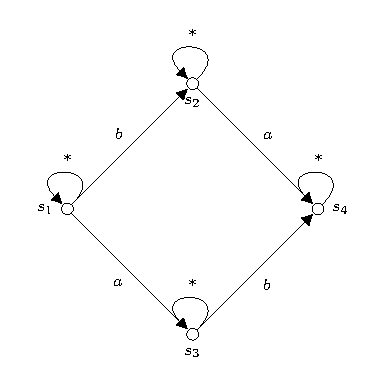
\includegraphics[scale=1.3]{Figures/2.Models-for-concurrency/idle-transition-system.pdf}
    %    \captionof{figure}[An idle transition system.]{A transition system with four states, $s_{1}, s_{2}, s_{3}$, and $s_{4}$, and eight transitions, two of which are labeled $a$, another two which are labeled $b$ and the remaining are loops labeled $*$. The paths with $a$ and $b$ represent the interleaving of two instructions. The interleaving is namely the permutation of all possible executions of these two instructions. While, transitions labelled $*$ refer to the possible inaction of a transition system.}
    %    \label{fig:idle-transition-system}
    %\end{figure}
    
    %This representation will also be reflected in our notation $\lambda : \mathcal{L} \rightarrow_{*} \mathcal{L}^{'}$, for a partial function $\lambda$ from $\mathcal{L}$  to $\mathcal{L}^{'}$. 
    %We define idle transition systems as in \cite{winskel95modelsCategory}.
    
    %\begin{definition}[Idle transition systems \cite{winskel95modelsCategory}]\label{def:idle-transition-system}
    %    Let $\mathcal{T}$ = ($\mathcal{S}, i, \mathcal{L}, Tran$) be a transition system. An idle transition of $\mathcal{T}$ consists of ($s, *, s$) and $s \in \mathcal{S}$ such that
    %    \begin{center}
    %        $Tran_{*} = Tran \cup \{(s,*,s)\ |\ s \in \mathcal{S}\}$.
    %    \end{center}
    %\end{definition}
    
    %We may also define morphisms between idle transition systems as follows:
    
    %\begin{definition}[Morphisms of idle transition systems \cite{winskel95modelsCategory}]\label{def:morphisms-of-idle-transition-system}
    %    Let $\mathcal{T}$ = ($\mathcal{S}, i, \mathcal{L}, Tran$) and $\mathcal{T}^{'}$ = ($\mathcal{S}^{'}, i^{'}, \mathcal{L}^{'}, Tran^{'}$) be transition systems. A morphism $f : \mathcal{T} \rightarrow \mathcal{T}^{'}$ is a pair $f = (\sigma, \lambda)$ where
    %    \begin{itemize}
    %        \item $\sigma : \mathcal{S} \rightarrow \mathcal{S}^{'}$
    %        \item $\lambda : \mathcal{L} \rightarrow \mathcal{L}^{'}$ are such that $\sigma(i)$ = $i'$ and $(s,a,s') \in Tran \Rightarrow (\sigma(s),\lambda(a),\sigma(s')) \in Tran^{'}_{*}$.
    %    \end{itemize}
    %\end{definition}
    
    %If a transition with label $a$ in $\mathcal{T}$ is undefined, then we want a transition with label $\lambda(a)$ in $\mathcal{T}^{'}$ to also be undefined. We will consider this as a transition representing inaction. With the introduction of idle transitions, morphisms on transition systems can be described as preserving transitions and the initial state. Lastly, we will also stress, as done in \cite{winskel95modelsCategory}, that an idle transition ($s, *, s$) represents inaction, and is to be distinguished from the action expressed by a transition ($s, a, s$) for a label \emph{a}. From now on, when referring to transition systems we mean idle transition systems with the extension of morphisms of transition systems considering idle transitions.
    
    We write $\allTS$ for the category of transition systems. Also, we name $\allTS_{E}$ its subcategory where we restrict to transition systems labeled on an alphabet $E$. The alphabet $E$ can be considered the same as the set of events $E$. The notion of transition systems and of morphisms between them is clearly related to directed graphs, labeled directed graphs, and labeled transition systems, but we will need to consider labeled cubical sets, which we will not do here. However, we will introduce precubical sets\footnote{In topology, the difference between cubical and precubical sets are similar to that of simplicial and presimplicial sets. The differences are subtle and will not be considered here. The distinction between cubical and precubical sets is presented in \cite{Goubault95PhDThesis}.} in Section \ref{sec:higher-dimensional-automata}.
\section{Event structures}
\label{sec:event-structures}
    Event structures were developed in \cite{winskel80events} as an attempt to bridge Petri net theory\footnote{Petri nets are considered a classical model of concurrency with important ideas to understand the current research. Research into Petri nets has been done extensively in models of concurrency literature. Hence, we will not investigate Petri nets. One can find an introduction to Petri nets in \cite{Petri73petrinets}, and one can also find a recent comparison to modern models of concurrency in \cite{Goubault18RelationshipsModelsForConcurrency}.} and domain theory. Specifically, event structures is considered an extension to stable families, which are sets of all events which may have occurred by some stage, or history, in the evolution of a process. An event structure represents a process. We will adopt the same notion as used by Winskel \cite{NielsenPW81eventstructures} and Van Glabbeek $\&$ Goltz \cite{GlabbeekP09configStruct} that families are called \emph{configuration structures}. This bridge between Petri nets and domain theory would allow concurrent systems to be translated into automata, or schedules, providing a schedule-automata duality \cite{NielsenPW81eventstructures, GlabbeekP09configStruct}.

 \begin{definition}[Event structure \cite{winskel95modelsCategory}]\label{def:event-structure}
    An event structure ($E, \leq, \#$) consists of a set $E$, of events which are partially ordered by $\leq$ (the causal dependency relation) and a binary, symmetric, irreflexive relation $\# \subseteq E \times E$ (the conflict relation) which satisfy
    
    \begin{itemize}
        \item $\{ e'\ |\ e' \leq e\}$ is finite (axiom of \emph{finite causes}), and
        \item $e \# e'$ and $ e' \leq e'' \Rightarrow e \# e''$ (conflict is \emph{hereditary}).
    \end{itemize}
    
    for all $e, e', e'' \in E$.
\end{definition}

Event structure is formally defined as a triple ($E, \#, \leq$), where $E$ is the set of events, $\# \subseteq E \times E$ is a conflict relation, and $\leq\ \subseteq E \times E$ is a partial order. If two events are in conflict, not both of them can happen in a single execution. Also, for the event $e$ to happen, all the events before it in the partial order must have happened. We consider that events $e$ and $e'$ are \emph{concurrent}, denoted $e\ co\ e'$, as follows:

    \begin{center}
        $e\ co\ e'\ $ iff $not\ ((e \leq e')$ or $(e' \leq e)$ or $e \# e'))$.
    \end{center}

If $e$ and $e'$ are not dependent on each other in either order and there is no conflict, then we may run $e$ and $e'$ concurrently.

The events in a prime event structure can be thought of as event occurrences without significant duration, in any history an event appear at most once. The relation of \emph{immediate} dependency $e \rightarrow e'$ means $e$ and $e'$ are distinct with $e \leq e'$ and also that there is no event in between.

 \begin{definition}[Configurations \cite{winskel95modelsCategory}]\label{def:configurations-event-structure}
    Let ($E, \leq, \#$) be an event structure, and its \emph{configurations}, $\mathcal{D}(E, \leq, \#)$, to consist of those subsets $x \subseteq E$ which are
    
    \begin{itemize}
        \item conflict-free: $\forall e, e' \in x . \neg (e \# e') and$
        \item downwards-closed: $\forall e, e' . e' \leq e \in x \Rightarrow e' \in x$.
    \end{itemize}
\end{definition}

As shown by Winskel in \cite[Proposition 18]{winskel95modelsCategory}, we can recover the important relations, such as conflict and partial order, associated with an event structure from its finite configurations. We will not present that here. We will, however, use configurations in our definition of a category of event structures. First, we have to introduce morphisms of event structures.

 \begin{definition}[Morphisms of event-structures \cite{winskel95modelsCategory}]\label{def:morphisms-event-structure}
    Let $ES$ = ($E, \leq, \#$) and $ES'$ = ($E', \leq', \#'$) be event structures. A \emph{morphism} from $ES$ to $ES'$ consists of a partial function $\eta : E \rightarrow_{*} E'$ on events which satisfies
    
    \begin{itemize}
        \item $x \in \mathcal{D}(ES) \Rightarrow \eta x \in \mathcal{D}(ES')$,
        \item $\forall e, e' \in x . \eta (e), \eta (e')$ are both defined, and
        \item $\forall e, e' \in x . \eta (e) = \eta (e') \Rightarrow e = e'$.
    \end{itemize}
\end{definition}

If we let ($E, \leq, \#$) be an event structure and let $x, x'$ be configurations, then we write $x \xrightarrow{e} x' \Leftrightarrow e \notin x$ and $x' = x \cup \{e\}$. From Proposition 19 in \cite{winskel95modelsCategory}, we have that two events $e$ and $e'$ are concurrent if and only if there exists configurations $x_1, x_2, x_3$ and $x_4$ such that we get the interleaving square, as shown in Figure \ref{fig:interleaving-square-event-structure}.

\begin{figure}[ht]
        \centering
        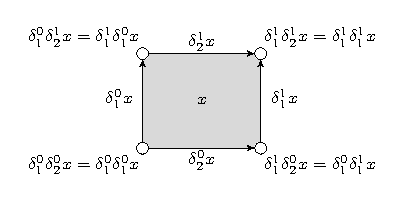
\includegraphics[scale=1.2]{Figures/2.Models-for-concurrency/event-structure/interleaving-square.pdf}
        \captionof{figure}[Configurations of an event structure]{An event structure with two concurrent events $e$ and $e'$ such that we get the configurations $x_{1}, x_{2}, x_{3}$, and $x_{4}$. The configurations generate the interleaving square because of the way the concurrent events $e$ and $e'$ form a square.}
        \label{fig:interleaving-square-event-structure}
\end{figure}

 We write $\allES$ for the category of event structures. Also, we name $\allES_{E}$ its subcategory where we restrict to event structures labeled on an alphabet $E$. The alphabet $E$ can be considered the same as the set of events $E$. Events are considered one side of a duality \cite{Pratt02eventStateDuality}, where automata is the other side. In Section \ref{sec:Chu-spaces} we will introduce Chu spaces \cite{gupta94phd_Chu}, which is a general framework where automata and schedules, with the Chu duality, can be converted into one another. Both automata and schedules have applications in different fields of computer science such as hardware design and analysis of asynchronous circuits, network diagnostics, distributed computation and logics of programs. 
\section{Summary}
    \label{sec:traditional-concurrency-summary}

    When considering the classification of concurrency models of Winskel et al. \cite{winskel94RelationshipsConcurrency}, we have that models are either simulating concurrency, known as \emph{interleaving}, or dealing directly with concurrency, namely \emph{non-interleaving}. The difference being that mutually exclusive occurrences are not distinguishable from truly independent ones in the former, but distinguishable in the latter.
    
    Interleaving models are not able to distinguish mutually exclusive events from truly independent events because the models depend on which events a process takes to be \emph{atomic} \cite[page 4]{Pratt86pomsets}. When we say atomic, we mean an indivisible action that must complete without interruption, in other words be considered instantaneous. If we suppose that an atomic event can be \emph{refined} in the same manner as how Pratt explains refinement of atomic actions in \cite{pratt91hda}, then the interleaving model can be seen to not have interleaved subactions. We will consider such a refinement as \emph{action refinement}. Action refinement is the method of developing a system by starting from a abstract specification, and gradually refining its action by providing more details \cite{Johansen16DecEventBasedConcurrencyRefinement, GlabbeekG89refinement}.
    
    % In the literature, it has shown that interleaving models are not well behaved under action refinement. \cite{x,y,z}.
    In the literature, it has been shown that interleaving models are not well behaved under action refinement \cite{GlabbeekG89refinement, GlabbeekG01refinement}. The model is forced to commit itself in advance to a particular level of granularity. For example, a programmer may give details on actions that, at the time, are regarded as atomic. However, at a future release the programmer may discover that the actions have substructures, see \cite[Example 1.1]{GlabbeekG89refinement}. The programmer cannot refine the action since it is atomic. There might be occurrences where the interleaving model can be seen not to have interleaved subactions. The failure  to interleave subactions is not characteristic of non-interleaving concurrency, but rather of a hidden assumption of excluded middle, or \emph{mutual exclusion} as it is more commonly known in concurrent processes \cite{Pratt00Sculptures}. We consider mutual exclusion to be where no actions can happen simultaneously, and must occur after each other.
    
    From our definition of transition systems, we are only able to simulate the parallel execution of two actions as the "\emph{interleaving}" of $ab$ or $ba$, see Figure \ref{fig:transition-system}. In the next chapter we will introduce asynchronous transition systems which extends the transition system to include an independence relation that is equipped to distinguish the mutual exclusion and independent occurrence of two events.
\chapter{An introduction to non-interleaving models of concurrency}
\label{chap:An introduction to models for true concurrency}
In this chapter we present non-interleaving models of concurrency that generalize the independence of two, or more, events. We present a geometric model of concurrency which is an algebraic structure able to capture the main characteristic of \emph{both} interleaving and non-interleaving models. We show both a state-based model, higher-dimensional automata, and an event-based model, ST-structures, capable of distinguishing an arbitrary number of events. Also, we present Chu spaces as a model able to present state-based and event-based models symmetrically, such that there is a way to present the event-state duality symmetrically. 

The models mentioned so far have been based on interleaving computation steps to capture all the possible behaviours of a concurrent system. Recall the interleaving square, in Figure \ref{fig:transition-system}, where we have four states $s_{1}$, $s_{2}$, $s_{3}$ and $s_{4}$ and four transitions, where two of the transitions are labeled $a$ and the other two transitions are labeled $b$. We see that these two actions $a$ and $b$ can be executed in either order, ending in the same state each way, such that $a$ and $b$ are mutually exclusive. By design, interleaving models depend on the notion of \emph{atomic} actions, that is, actions that are indivisible.

The assumption of atomic actions is reasonable for events that are mutually exclusive, meaning they cannot occur simultaneously. For example, a vending machine able to provide a single item at a time, like a snack or a beverage. If we want two items, such as a chocolate and a beverage, from the vending machine, then either the chocolate will be released followed by the beverage or first the beverage followed by the chocolate. However, for events that are truly independent, such as a vending machine able to provide two, or more, items at a time, then their order of occurrence would be rendered irrelevant $-$ two items would be released at the same time from the vending machine. Models that only allow interleaving are unable to distinguish these two vending machine. Instead, we will consider the non-interleaving models of concurrency, such as \emph{asynchronous transition systems} \cite{winskel95modelsCategory} and \emph{higher-dimensional automata} \cite{pratt91hda}, \emph{ST-structures} \cite{Johansen16STstruct} and \emph{Chu spaces} \cite{gupta94phd_Chu}, which are able to distinguishing between these two vending machines. Thus, we allow receiving multiple items after each other, or all at the same time. Going further, we may even have a combination of the alternatives.

For didactic and historical reasons, we will review asynchronous transition systems where we introduce an independence relation between the occurrence of events. The independence relation is able to express the mutual exclusion and non-interleaving of two events. Asynchronous transition systems may be considered a bridge between transition systems, used up until now, and the higher-dimensional automata, introduced in Section \ref{sec:higher-dimensional-automata}. Higher-dimensional automata are expressive and can encode the independence of an arbitrary number of events, rather than only pairs of events.

Higher-dimensional automata are \emph{algebraic structures} which can be interpreted geometrically, roughly as topological spaces with a sense of direction to incorporate a notion of irreversible time. A topological space with a sense of direction makes it possible to determine the order of an execution. Intuitively, a higher-dimensional automaton is an automaton with nicely incorporated squares, cubes and higher-dimensional cubes, which represent the independence of events. A main characteristic of higher-dimensional automata is to be able to capture what happens \emph{during} an execution. ST-structure is the event-based counterpart of higher-dimensional automata which is able to precisely identify events, and also capture what happens during an execution. As shown by Johansen in \cite{Johansen16STstruct}, higher-dimensional automata cannot precisely identify events. For example, the asymmetric conflict shown in \cite[Figure 5]{Johansen16STstruct} and presented in Section \ref{sec:st-structure-and-hda}. However, we may faithfully represent the asymmetric conflict as a ST-structure.
\section{Asynchronous transition systems}
\label{sec:asynchronous-transition-systems}

    Asynchronous transition systems were introduced independently by Bednarczyk \cite{bed88CategoriesAsynchSystems} and Shields \cite{Shields84}. They extend transition systems by including a \emph{binary} independence relation between the occurrence of events. In this model, transitions are events bearing this independence relation. Asynchronous transition systems can be viewed as asynchronous graphs, whose vertices are states and whose edges are transition between states. Transitions take the commutation between events into consideration \cite[Section 3.3]{Fajstrup16DirectedAlgebraicTopologyConcurrency}. If two events commute, then these may be executed at the same time. Meaning that we can consider two transitions of events as a single transition with two events.
    
    \begin{definition}[Asynchronous transition system \cite{winskel95modelsCategory}]\label{def:asynchronous-transition-system}
        An \emph{asynchronous transition system} is a tuple ($\mathcal{S},i,E,\mathcal{I},Tran$) where
        \begin{itemize}
            \item ($\mathcal{S},i,E,Tran$) is a transition system and
            \item $\mathcal{I} \subseteq E \times E$ is an irreflexive symmetric relation, called the independence relation, such that:
            
            \begin{enumerate}
                \item $a \in E \Rightarrow \exists s, s' \in \mathcal{S}, (s,a,s') \in Tran$.
                \item $(s,a,s') \in Tran \wedge (s,a,s'') \in Tran \Rightarrow s' = s''$.
                \item $a\mathcal{I}b \wedge (s_{1},a,s_{2}) \in Tran \wedge (s_{1}, b, s_{3}) \in Tran \Rightarrow \exists u, (s_{2},b,u) \in Tran \wedge (s_{3},a,u) \in Tran$.
                \item $a\mathcal{I}b \wedge (s_{1},a,s_{2}) \in Tran \wedge (s_{2}, b, u) \in Tran \Rightarrow \exists s_{3}, (s_{1},b,s_{3}) \in Tran \wedge (s_{3},a,u) \in Tran$.
            \end{enumerate}
        \end{itemize}
    \end{definition}
    
    Condition (1) says every event should appear as a transition. Condition (2) says that transitions with an event from a state has to be unique, meaning that the transition system should be deterministic. Condition (3) and (4), are pictured respectively in Figure \ref{fig:condition-3-asynchronous-transition-systems} and \ref{fig:condition-4-asynchronous-transition-systems}, exhibiting the transitions of events bearing the independence relation that deals with independent events.
    
    \begin{figure}[ht]
        \centering
        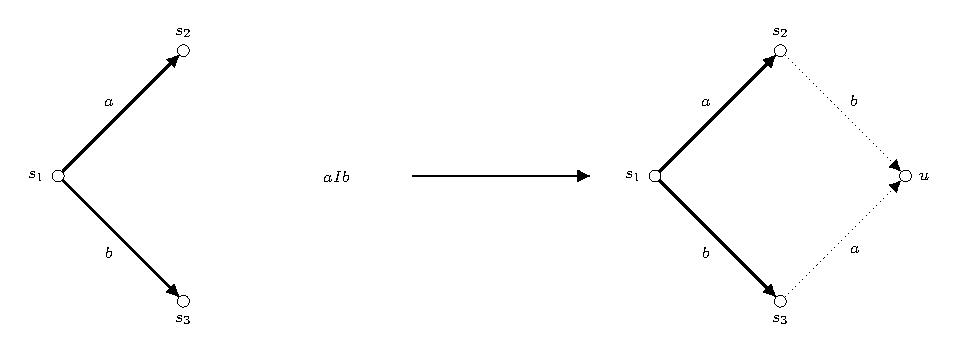
\includegraphics[scale=1]{Figures/2.Models-for-concurrency/Asynchronous-transition-system-condition3.pdf}
         \captionof{figure}[Condition (3) for asynchornous transition systems]{Condition (3) for asynchronous transition systems, where the right-hand side shows how to interpret two independent events coming from a common state. If two events, $a$ and $b$, occur independently from a common state $s$, then they should be able to form the right-hand side.}
        \label{fig:condition-3-asynchronous-transition-systems}
    \end{figure}
    
    \begin{figure}[ht]
        \centering
        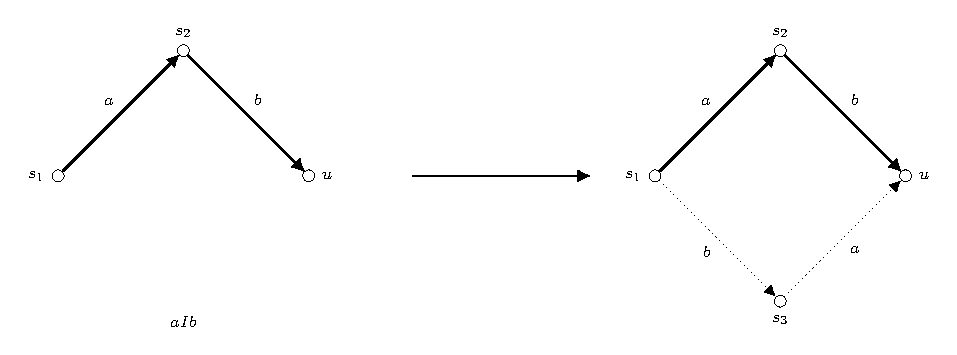
\includegraphics[scale=1]{Figures/2.Models-for-concurrency/Asynchronous-transition-system-condition4.pdf}
        \captionof{figure}[Condition (4) for asynchronous transition systems]{Condition (4) for asynchronous transition systems, where the right-hand side shows how to interpret two independent events occurring immediately after each other. If two events, $a$ and $b$, occur one immediately after the other, then they should be able to occur with their order interchanged.}
        \label{fig:condition-4-asynchronous-transition-systems}
    \end{figure}
    
     Morphisms between asynchronous transition systems are morphisms between their underlying transition systems which preserve the additional relations of independence.
    
    \begin{definition}[Morphisms of asynchronous transition system \cite{winskel95modelsCategory}]\label{def:morphisms-asynchronous-transition-system}
       Let $\mathcal{T} = (\mathcal{S},i,E,\mathcal{I},Tran)$ and $\mathcal{T}^{'} = (\mathcal{S}^{'},i^{'},E^{'},\mathcal{I}^{'},Tran^{'})$ be asynchronous transition systems. A morphism $\mathcal{T} \rightarrow \mathcal{T}^{'}$ is a morphism of transition systems
       
       \begin{center}
            $(\sigma, \lambda) : (\mathcal{S},i,E,Tran) \rightarrow (\mathcal{S}^{'},i^{'},E^{'},Tran^{'})$
       \end{center}
       
       such that
       
       \begin{center}
           $a\mathcal{I}b$ and $\lambda(a), \lambda(b)$ are both defined $\implies$ $\lambda(a)\mathcal{I}\lambda(b)$.
       \end{center}
    \end{definition}
    
    Morphisms of asynchronous transition systems compose as morphisms between their underlying transition systems. We can turn asynchronous transitions systems into a category, written $\allATS$. The category of asynchronous transition systems restricted over the events $E$ is named $\allATS_{E}$.
    
    In interleaving models for concurrency, the number of executions grow exponentially with the size of the program. Every possible execution of a program must be considered, which is not feasible in practice. Non-interleaving models take the commutation of instructions into account, that is, allowing instructions to be executed at the same time. By commuting instructions, it minimizes the number of possible executions of a program by considering certain instructions to be equivalent.
    
    From the independence relation, we can observe that many of the schedules are equivalent in the sense that one can be obtained from the other by permuting independent instructions. Furthermore, such equivalent executions will always lead to the same result. Consequently, if one of those executions can be shown not to lead to an error, neither will any other execution which is equivalent to it.
    
    An independence relation is able to deal directly with concurrency. However, the relation is binary meaning that at most two events can be distinguished. To be able to distinguish an arbitrary number of events, we could extend the independence relation to be an $n$-$ary$ relation. However, this relation should be interpreted as a tractable algebraic theory, which has shown to be challenging.
\section{Higher-dimensional automata}
\label{sec:higher-dimensional-automata}

    The generalization of independence to $n$ events has lead to a geometric model for concurrency, studied by Pratt and van Glabbeek \cite{pratt91hda, Pratt00Sculptures, Glabbeek06HDA}. Pratt named this model Higher-Dimensional Automata (HDA) \cite{pratt91hda}. With higher-dimensional automata we can distinguish between the execution of $n$ non-interleaving concurrent events and of $n$ mutually exclusive events. Higher-dimensional automata are considered to be of high expressive power because of their property to distinguish $n$-events \cite{Kahl2013TheHG}. Hence, providing a generalization of differences, and common features, of various other models of concurrency, as done in \cite{Glabbeek06HDA} and \cite{Goubault18RelationshipsModelsForConcurrency}. Higher-dimensional automata also retain the state-based view and model the interleaving square with its interior filled, shown in Figure \ref{fig:HDA-filled-interleaving-square}. 
    
   A higher-dimensional automaton is a precubical set that encodes the independence of events by \emph{mappings}. Intuitively, we may consider a precubical set as $n$-dimensional cubes \cite{Fajstrup16DirectedAlgebraicTopologyConcurrency} together with their faces $-$ each $n$-dimensional cube has $2n$ faces. In other words, a front and a back face in each direction $i$ with $0 \leq i < n$. Mappings are families of functions that identify these faces, we call these \emph{face maps}. Face maps that satisfy the \emph{precubical identity} \cite{Fahrenberg05PhD, Fajstrup05DipathsInCubicalComplex, Fajstrup06AlgebraicTopologyConcurrency, Goubault2001TopologicalDeformHDA, goubault2003SomeGeometricPerspectives} are able to interpret the independence of events. In the concurrency theory literature, we find that the precubical identity is named the \emph{cubical law} \cite{Glabbeek06HDA, Johansen16STstruct}, since applications of algebraic topology are still being investigated in concurrency theory. Here, we will follow the topological notion, and use the naming precubical identity.

    Intuitively, the precubical identity is considered to be the idea of "\emph{filling in holes}" of a $n$-dimensional cube \cite[Section 2]{pratt91hda}. This notion is shown in Figure \ref{fig:HDA-filled-interleaving-square}, where the interior of the interleaving square is filled. With higher-dimensional automata we are able to capture the main characteristic of both transition systems and asynchronous transition systems by the notion of "\emph{filling in holes}".
    
  
    \begin{definition}[Precubical set]
        \label{def:precubical-set}
         A \emph{precubical set} is a graded set $\mathcal{X}= \bigcup_{ n\in \Nat} \mathcal{X}_n$, with $\mathcal{X}_n\cap \mathcal{X}_m= \emptyset$ for $n\ne m$, together with mappings $s_{ k, n}, t_{ k, n}:\mathcal{X}_n\to \mathcal{X}_{ n- 1}$, with $1\leq k\leq n$, satisfying the \emph{precubical identities}
         
         %$\delta_{ k, n}^\nu:\mathcal{X}_n\to \mathcal{X}_{ n- 1}$, $k = 1,\dots, n$, $\nu \in \{0, 1\}$, satisfying the \emph{precubical identity}
        
        \begin{equation*}
            \alpha_{ k, n- 1} \beta_{ \ell, n}= \beta_{ \ell- 1, n- 1} \alpha_{ k, n} \qquad(1 \leq k< \ell \leq n)
        \end{equation*}
        for $\alpha, \beta\in\{ s, t\}$.
    \end{definition}
    
    A \emph{graded} set is a \emph{family of sets} where its elements are $n$-cells. A \emph{family of sets} is the disjoint union of these $n$-cells, $\mathcal{X}_n\cap \mathcal{X}_m= \emptyset$ for $n\ne m$. In the beginning of this Section, we called these $n$-cells for $n$-dimensional cubes. The naming $n$-dimensional cubes comes from Fajstrup et al. \cite{Fajstrup16DirectedAlgebraicTopologyConcurrency}, where $n$-dimensional cubes are precubical sets together with their faces. In this thesis, we will call elements of $\mathcal{X}_n$ for $n$-cells,  or simply cells, even though there are different names for these elements such as \emph{$n$-dimensional cubes} \cite{Pratt00Sculptures, Fajstrup16DirectedAlgebraicTopologyConcurrency}, \emph{$n$-transitions} \cite{Goubault95PhDThesis} and \emph{hypercubes} \cite{Glabbeek06HDA}. If $x \in \mathcal{X}_n$, then we say that $x$ is of dimension $n$ and is written $dim x = n$.
    
    The mappings $s_{ k, n}$ and $t_{ k, n}$  are called \emph{face maps}, and we will usually omit the extra subscript $n$ and simply write $s_k$ and $t_k$. Face maps are families of functions that identify the faces of the $n$-cells, in the same manner as described with $n$-dimensional cubes. Families of functions are usually considered as a set of functions whose equations have a similar form. However, in this context we will interpret them geometrically as faces of a cube.
    
    Each $n$-cell $x \in \mathcal{X}_n$ has \emph{$n$ lower faces $s_1 x,\dotsc, s_n x$} and \emph{$n$ upper faces $t_1 x,\dotsc, t_n x$}, and the precubical identity expresses the fact that ($n-1$)-faces of an $n$-cell meet in common ($n-2$)-faces, see Figure \ref{fig:precubical-set-interleaving-square-preidentity}.
    
    Figure \ref{fig:precubical-set-interleaving-square-geometric} and \ref{fig:precubical-set-interleaving-square-preidentity} represent a 2-cell showing both the four faces $s_1 x$, $t_1 x$, $s_2 x$, $t_2 x$ and the four possible mappings of the precubical identity. Figure \ref{fig:precubical-set-interleaving-square-geometric} is more of a geometrical picture of the 2-cell with its interior filled.
    
    \begin{figure}[ht]
        \centering
        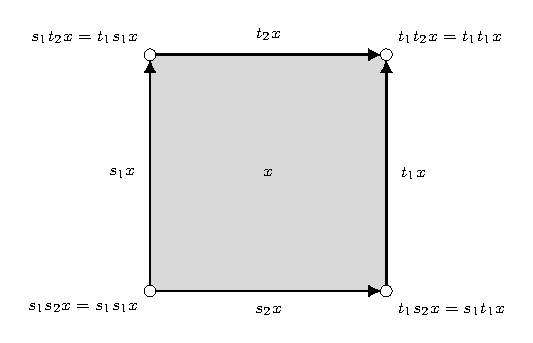
\includegraphics[scale=1.2]{Figures/3.An-introduction-to-non-interleaving-models-for-concurrency/precubical-square/cubical-law-2-cell-geometrical.pdf}
         \captionof{figure}[Geometric representation of a 2-cell]{We have a geometrical picturing of the 2-cell with its interior filled, four faces $s_1 x$, $t_1 x$, $s_2 x$, $t_2 x$ and four corners representing the mappings of the precubical identity.}
        \label{fig:precubical-set-interleaving-square-geometric}
    \end{figure}
    
    While, Figure \ref{fig:precubical-set-interleaving-square-preidentity} shows how the four mappings of the precubical identity is satisfied, and the fact that 1-faces of a 2-cell meet in common 0-faces.
    
    \begin{figure}[ht]
        \centering
        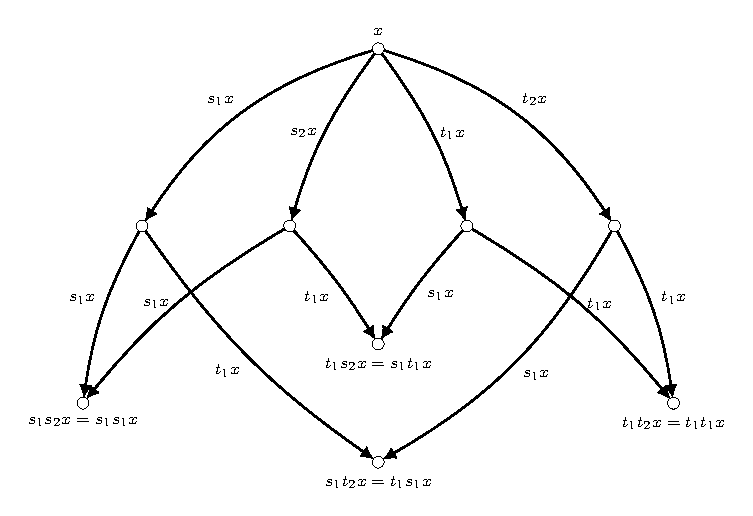
\includegraphics[scale=1]{Figures/3.An-introduction-to-non-interleaving-models-for-concurrency/precubical-square/cubical-law-2-cell-preidentity.pdf}
         \captionof{figure}[2-cell satisfying the precubical identities]{We have a 2-cell showing the four faces $s_1 x$, $t_1 x$, $s_2 x$, $t_2 x$ as edges and the four mappings of the precubical identity as the bottom nodes of the 2-cell.}
        \label{fig:precubical-set-interleaving-square-preidentity}
    \end{figure}
    
    We need a notion of \emph{morphisms} between precubical sets to be able to study the relationship between higher dimensional automata. From Section \ref{sec:ordinary-transition-systems}, we have that morphisms are considered to be simulations. Morphisms as simulation was an idea from Winskel and Nielsen in \cite{winskel95modelsCategory}. We want to extend morphisms to be structure-preserving maps that preserve orientation, shape, and time \cite[Section 2.2]{Goubault95PhDThesis}.
    
    Preserving orientation is addressed by \emph{directed} topology, where the object of study are topological spaces that have a sense of direction. Specifically, a topological space with a directed variant to incorporate the notion of irreversible time. Topology is a branch in mathematics that studies geometric shapes, and directed topology considered these geometric shapes to have a sense of direction. Shapes are preserved if we can present the geometry, we are interested in, as unions of \emph{points, segments, squares, cubes, ..., $n$-dimensional cubes} as collections of \emph{$n$-cells} ($n \in \mathbb{N}$). Preserving time means that we can reason about the directed variant and that every transition is mapped onto a transition.
    
    \begin{definition}[Morphism of precubical sets]
        \label{def:morphism-of-precubical-set}
        Morphisms $f: \mathcal{X}\to \mathcal{Y}$ of precubical sets are graded functions $f=\{ f_n: \mathcal{X}_n\to \mathcal{Y}_n\}_{ n\in \Nat}$ which commute with the face maps:
        
        \begin{equation*}
            \alpha_k\circ f_n= f_{ n- 1}\circ \alpha_k \qquad\ \text{for all}\ n\in \Nat,\ k\in\{ 1,\dots, n\},\ \text{and}\ \alpha\in\{ s, t\}.
        \end{equation*}
    \end{definition}

    Higher-dimensional automata are simply defined in terms of the precubical sets, and the relationship between higher-dimensional automata is described by the morphisms of the underlying precubical sets. Every figure presented thus far, may be considered as a higher-dimensional automata. We will from now on refer to the previous figures as higher-dimensional automata even though we first introduced them as transition systems, asynchronous transition systems and $n$-cells.
    
    \begin{definition}[Higher-dimensional automata \cite{Glabbeek06HDA, Johansen16STstruct}]
        \label{def:higher-dimensional-automata}
        A precubical set $\mathcal{H} = (\mathcal{Q},s,t)$ is a precubical set $\mathcal{Q}$ together with $s$ and $t$ being the collection of all the face maps, that is, for all $n$. 
        
        A higher-dimensional automata is a tuple $(\mathcal{Q}, s, t, l, \mathcal{I}, \mathcal{F})$ over an alphabet $\Sigma$ such that $l(s_i(q)) = l(t_i(q))$ for all $q \in \mathcal{Q}_2$ and $i \in \{1,2\}$, and with a designated initial cell $\mathcal{I} \in \mathcal{Q}_0$ and $\mathcal{F} \subseteq \mathcal{Q}_0$ final cells.

    \end{definition}

    The concurrent execution of a higher-dimensional automata is modeled by including the two-dimensional surface. Intuitively, a concurrent execution can be seen as moving across the surface such that the execution preserves the directed variant, that is, to incorporate a notion of irreversible time. This is pictured in Figure \ref{fig:HDA-filled-interleaving-square}. 
    
    \begin{figure}[ht]
        \centering
        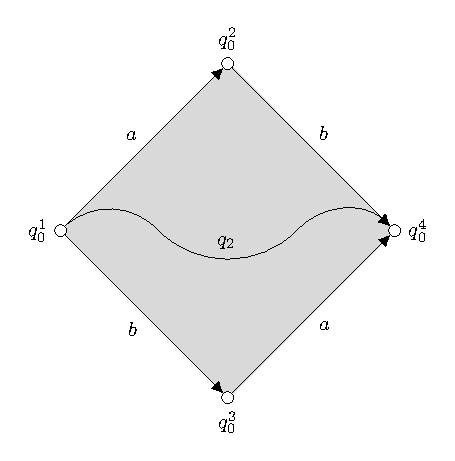
\includegraphics[scale=1.2]{Figures/3.An-introduction-to-non-interleaving-models-for-concurrency/HDA_filled_interleaving_square/filled-interleaving-diamond.pdf}
         \captionof{figure}[Filled interleaving square]{Example of a HDA with four states, $q^1_0, q^2_0, q^3_0$ and $q^4_0$, four transitions, two of which are labeled $a$ and the other two are labeled $b$, and a surface, $q_2$. The surface represents the notion of "filling in holes" \cite[Section 2]{pratt91hda}, which is a continuous deformation of instructions $ab$ into $ba$, or vice versa.}
        \label{fig:HDA-filled-interleaving-square}
    \end{figure}
    
    A computation is a path in this higher-dimensional automaton.
    
    \begin{definition}[Paths in HDAs \cite{Johansen16STstruct}]\label{def_paths_HDA}
        \label{def:paths-in-HDAs}
        A \emph{single step} in a HDA is either
        \begin{enumerate}
            \item $q_{n-1}\transition{s_{i}}q_{n}$ with $s_{i}(q_{n})=q_{n-1}$ or 
            \item $q_{n}\transition{t_{i}}q_{n-1}$ with $t_{i}(q_{n})=q_{n-1}$, 
        \end{enumerate}
        \noindent where $q_{n}\in \mathcal{Q}_{n}$ and $q_{n-1}\in \mathcal{Q}_{n-1}$ and $1\leq i\leq n$. 

        A \emph{path} $\pi\defequal q^{0}\transition{\alpha^{1}}q^{1}\transition{\alpha^{2}}q^{2}\transition{\alpha^{3}}\dots$ is a sequence of single steps $q^{j}\transition{\alpha^{j+1}}q^{j+1}$, with $\alpha^{j}\in\{s,t\}$. We say that $q\in\pi$ iff $q=q^{j}$ appears in one of the steps in $\pi$.  The first cell in a path is denoted $\startPath{\pi}$ and the ending cell in a finite path is $\finishPath{\pi}$. 
    \end{definition}
    
    The markings of the steps by $s$ may be seen as going from a lower cell to a higher cell, and steps by $t$ as the opposite, in the higher dimensional automaton. In many of the later proofs it is though useful to have the exact map easily visible, namely, the index that the step uses, rather than explicitly assuming the index every time. If there is no $\finishPath{\pi}$, then the path is infinite. When the index is not important we write $\transition{s}$ or $\transition{t}$.
    
    \begin{definition}[Histories for $\HDA$s \cite{Johansen16STstruct}]
    \label{def:histories-for-HDA}
    
        In a $\HDA$ two paths are \emph{adjacent}, denoted $\pi\adjacentHDA\pi'$, if one can be obtained from the other by replacing, for $q,q'\in \mathcal{Q}$ and $i<j$,
        
        \begin{enumerate}
            \item a segment $\transition{s_{i}}q\transition{s_{j}}$ by $\transition{s_{j-1}}q'\transition{s_{i}}$, or
            \item a segment $\transition{t_{j}}q\transition{t_{i}}$ by $\transition{t_{i}}q'\transition{t_{j-1}}$, or
            \item a segment $\transition{s_{i}}q\transition{t_{j}}$ by $\transition{t_{j-1}}q'\transition{s_{i}}$, or
            \item a segment $\transition{s_{j}}q\transition{t_{i}}$ by $\transition{t_{i}}q'\transition{s_{j-1}}$.
        \end{enumerate}

        Two finite paths are \textit{l-adjacent} $\pi\ladjacentHDA{l}\pi'$ when the segment replacement happens at position $l+1$; that is, $q$ is the $l+1$ cell in the path. \emph{Homotopy} is the reflexive and transitive closure of adjacency. Two homotopic paths are denoted $\pi\homotopicHDA\pi'$ and share their respective start and end cells. The homotopy class of a rooted path is denoted $\homotopyClass{\pi}$. A homotopy class with end cell $q$ is said to be \emph{a history of $q$}. One cell may have several histories, as is the case with the interleaving square $\HDA$ from Figure~\ref{fig:HDA-filled-interleaving-square}. Whenever a cell has a unique history we use the notation $\homotopyClass{q}$, instead of $\homotopyClass{\pi}$ with $\finishPath{\pi}=q$.
    \end{definition}

    Homotopy is defined for all paths such that a cell of higher dimension has a history in the same way that the inside of a square has a history. The homotopy is provided by Johansen in \cite{Johansen16STstruct}, where the homotopy is different compared to the definition in \cite[Section 1.6]{Goubault18RelationshipsModelsForConcurrency} because not only the state cells of dimension $0$, that is, vertices that form the corners of a cube, have histories, but also cells of higher dimensions.
    
    History unfoldings of process graphs have been defined by Van Glabbeek in \cite[Section 3]{Glabbeek96HistoryUnfolding}. Inspired by the definition of history unfoldings of process graphs, we will define the same notion for higher-dimensional automata. Johansen in \cite{Johansen16STstruct}, provides a definition of history unfolding for higher-dimensional automata which can be correlated with the definition of unfoldings from \cite{Glabbeek96HistoryUnfolding}. Also, alternative definitions of unfoldings for $\HDA$ can be found in \cite{Fahrenberg05PhD, Fahrenberg15PartialHDA}.

    \begin{definition}[History unfolding for HDAs]\label{def_unfolding_history} 
        The \emph{history unfolding} of a higher dimensional automaton $\mathcal{H}$ is a $\HDA$ denoted $\unfolding(\mathcal{H})$, respecting the cubical laws, as shown in \cite[Proposition 3.30]{Johansen16STstruct}, and given by:
        
        \begin{itemize}
            \item $Q_{n}^{\unfolding(\mathcal{H})}$ is the set of histories that end up in cells on level $Q_n$ of $\mathcal{H}$;
            \item has the labelling copied from $\mathcal{H}$: $l^{\unfolding(\mathcal{H})}(\homotopyClass{\pi})=l^{H}(\finishPath{\pi})$;
            \item initial cell the empty rooted history;
            \item the $s/t$ maps are built from the corresponding maps between the end cells of the histories: 
                \[
                    s_{i}(\homotopyClass{\pi})=\homotopyClass{\pi'}\mbox{\ \ \ iff\ \ \ }s_{i}(q)=q'\wedge \pi'\transition{s_{i}}\pi\wedge \finishPath{\pi'}=q'\wedge \finishPath{\pi}=q;
                \]
                \[
                    t_{i}(\homotopyClass{\pi})=\homotopyClass{\pi'} \mbox{\ \ \ iff\ \ \ } t_{i}(q)=q' \wedge \pi\transition{t_{i}}\pi' \wedge \finishPath{\pi'}=q'\wedge \finishPath{\pi}=q.
                \]
        \end{itemize}
    \end{definition}
    
    The notion of \emph{unfolding} removes iteration and is commonly used to turn a complicated model such as higher-dimensional automata into a simpler, but potentially infinite one. Unfolding is important in relation to the sculpting method introduced in Chapter \ref{chap:sculpting-in-concurrency}. For HDA this picture is more complicated.  Figure~\ref{fig:HDA-broken-box} (left) shows a simple HDA which is a sculpture. However, we will show that its unfolding (right) is \emph{not} a sculpture.

    \begin{definition}[Morphism of HDAs \cite{Johansen16STstruct}]
        \label{def:isomorphism-of-higher-dimensional-automata}
        A morphism between two \emph{HDA}s, $f : \mathcal{H} \rightarrow \mathcal{H}'$ is a dimension preserving map between their cells $f : \mathcal{Q} \rightarrow \mathcal{Q}'$, such that:
        
        \begin{enumerate}
            \item the initial cell is preserved: $f(\mathcal{I}) = \mathcal{I}'$
            \item the labelling is preserved: $l'(f(q_1)) = l(q_1)$ for all $q_1 \in \mathcal{Q}_1$,
            \item the mappings are preserved, for any $q_n \in \mathcal{Q}_n$ and $1 \leq i \leq n$:
            \begin{itemize}
                \item $s'_i(f(q_n)) = f(s_i(q_n))$ and
                \item $t'_i(f(q_n)) = f(t_i(q_n))$.
            \end{itemize}
        \end{enumerate}
        
        When a morphism is bijective we call it isomorphism. Two HDAs are isomorphic, denoted $\mathcal{H} \cong \mathcal{H}'$, when there exists an isomorphism between them.
    \end{definition}

    We write $\allHDA$ for the category of higher-dimensional automata, where the object of the category are higher-dimensional automata and morphisms are as defined in Definition \ref{def:isomorphism-of-higher-dimensional-automata}.
    
    In the definition of precubical sets, we consider them to be non-degenerate. Many of the results from this thesis assumes higher-dimensional automata to be non-degenerate. Also, we consider the directed variant, mentioned so far, to be higher-dimensional automata that are acyclic. Johansen in \cite{Johansen16STstruct}, defines these notions for higher dimensional automata:
    
    \begin{definition}[Acyclic and non-degnerate HDAs \cite{Johansen16STstruct}]
        \label{def:acyclic-and-non-degenerate-higher-dimensional-automata}
        A higher-dimensional automata is called acyclic if no path visits a cell twice. A higher-dimensional automata is non-degenerate if for any cell $q$ all its faces exist and are different, in the sense of $\forall i \neq j : \alpha_i(q) \neq \beta_i(q) \wedge \alpha , \beta \{s,t\}$, no two transitions with the same label share both their end states.
    \end{definition}
    
    The notion of acyclic does not allow cycles, or loops, in the higher-dimensional automata, and the notion of non-degeneracies is related to the underlying precubical sets\footnote{In topology, The distinction between non-degeneracies and degeneracies are subtle and will not be considered here. In \cite{Goubault95PhDThesis}, the  distinction between non-degeneracies and degeneracies is considered.}. The restriction on higher-dimensional automata being non-degenerate is similar to that of Fajstrup et al. \cite{Fajstrup16DirectedAlgebraicTopologyConcurrency} and that of van Glabbeek \cite{Glabbeek06HDA}. Also, the restriction above is the same for precubical sets where two opposite s-maps and t-maps can be equal, such that $s_i(q) = t_i(q)$ is allowed. We assume all s-maps and t-maps are to be total, as done in \cite{Johansen16STstruct}. A study of partial higher-dimensional automata, where s-maps and t-maps are partial, has been considered by Fahrenberg in \cite{Fahrenberg15PartialHDA}.
\section{ST-structures}
\label{sec:ST-structures}
    
    ST-structures are first introduced by Johansen in \cite{Johansen16STstruct}. They are an extension of \emph{configuration structures} \cite{GlabbeekP95config} and \emph{unrestricted} event structures \cite{GlabbeekP09configStruct}. 
    
    \begin{figure}[ht]
        \centering
        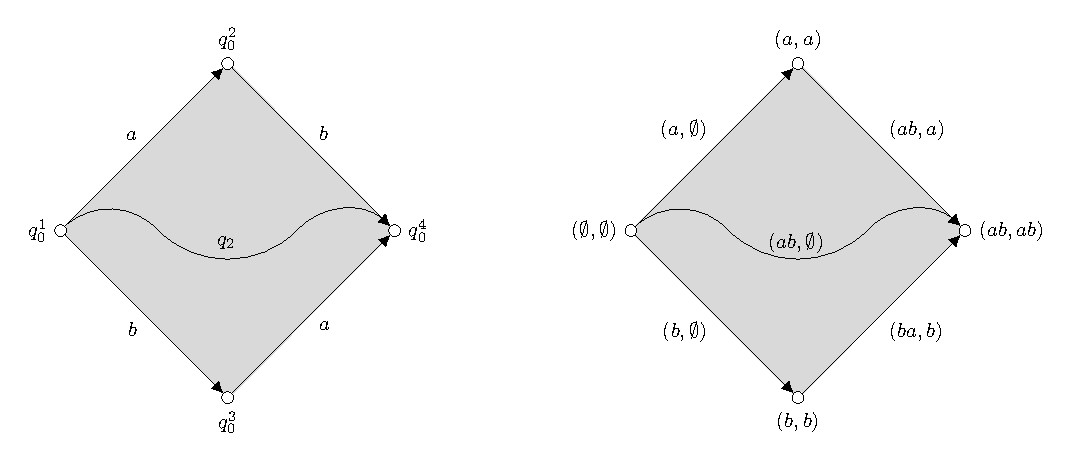
\includegraphics[scale=0.9]{master_thesis/Figures/3.An-introduction-to-non-interleaving-models-for-concurrency/ST-structure/st-structure-interleaving-square.pdf}
         \captionof{figure}[ST-structure]{Example of a higher-dimensional automaton with two concurrent events labelled by $a$ and $b$: with a geometrical picture of the higher-dimensional automaton (left) and of the ST-structure (right).}
        \label{fig:st-structure-interleaving-square}
    \end{figure}
    
    In the case of configuration structures and event structures, we have that the classical notion of concurrency, causality, and conflict are not interdefinable. In the case of higher-dimensional automata these notions can be interdefinable. In Chapter \ref{chap:Relationship with other models of true concurrency}, we relate ST-structures to higher-dimensional automata by identifying a corresponding class of ST-structures with the particular property of \emph{adjacent-closure}. With the adjacent-closure property, ST-structures are able to capture the higher-dimensional case of the notions of concurrency, causality and conflict. We will use the same notation and definitions as Johansen in \cite{Johansen16STstruct}.
    
    \begin{definition}[ST-configuration \cite{Johansen16STstruct}]
        \label{def:st-configuration}
        An ST-configuration over some set $E$ of events is a pair of finite sets ($\mathcal{S},\mathcal{T}$) ($\mathcal{S}, \mathcal{T} \subseteq E$) respecting the property:
        
        \begin{center}
            (start before terminate) $\mathcal{T} \subseteq \mathcal{S}$.
        \end{center}
    \end{definition}
    
    In the following, $\mathcal{S}$ contains the events that have started and $\mathcal{T}$ the events that have terminated. In the current ST-configuration, we see the events $\mathcal{S} \setminus \mathcal{T}$ as being executed \emph{concurrently}. We will call $| \mathcal{S} \setminus \mathcal{T} |$ the concurrent degree of this ST-configuration, similar to how we defined dimensions for higher-dimensional automata. The notion of degree, and dimension, is the main characteristic captured by ST-structures which is found in higher-dimensional automata, but not found in classical event-based models like configuration structures or event structures. In ST-structures, an event can be seen to have started and not terminated yet, capturing the notion of \emph{duration}.
    
    \begin{definition}[ST-structures \cite{Johansen16STstruct}]
        \label{def:st-structures}
        An ST-configuration structure (also called ST-structure) is a tuple $ST$ = ($E, ST, l$) with ST a set of ST-configurations over $E$ satisfying the constraint:
        
        \begin{center}
            if ($\mathcal{S},\mathcal{T}$) $\in$ ST then ($\mathcal{S},\mathcal{S}$) $\in$ $ST$,
        \end{center}
    
    and $l:E$ $\rightarrow \Sigma$ a labelling function with $\Sigma$ the set of labels. we often omit the set of events $E$ from the notation when there is no danger of confusion.
    \end{definition}
    
    Intuitively, the constraint above ensures that every event that is represented, and that has also started, has to be terminated. We denote $\mathbb{S} \mathbb{T}$ as the set of all ST-structures.
    
    \begin{definition}[Stable ST-structures \cite{Johansen16STstruct}]
        \label{def:stable st-structures}
        A ST-structure ($E, ST,l$) is called:
        
        \begin{enumerate}
            \item rooted iff ($\emptyset$,$\emptyset$) $\in ST$;
            \item connected iff for any non-empty ($\mathcal{S},\mathcal{T}$) $\in ST$, either \\
            $\exists$e $\in$ $\mathcal{S}$ : ($\mathcal{S}\setminus e, \mathcal{T}$) $\in ST$ or $\exists$e $\in \mathcal{T}$ : ($\mathcal{S}, \mathcal{T}\setminus e$) $\in ST$;
            \item closed under bounded unions iff for any ($\mathcal{S},\mathcal{T}$),($\mathcal{S}',\mathcal{T}'$),($\mathcal{S}'',\mathcal{T}''$) $\in ST$ if ($\mathcal{S},\mathcal{T}$) $\cup$ ($\mathcal{S}',\mathcal{T}'$) $\subseteq$ ($\mathcal{S}'',\mathcal{T}''$) then ($\mathcal{S},\mathcal{T}$) $\cup$ ($\mathcal{S}',\mathcal{T}'$) $\in ST$;
            \item closed under bounded intersection iff for ($\mathcal{S},\mathcal{T}$),($\mathcal{S}',\mathcal{T}'$),($\mathcal{S}'',\mathcal{T}''$) $\in ST$ if ($\mathcal{S},\mathcal{T}$) $\cup$ ($\mathcal{S}',\mathcal{T}'$) $\subseteq$ ($\mathcal{S}'',\mathcal{T}''$) then ($\mathcal{S},\mathcal{T}$) $\cap$ ($\mathcal{S}',\mathcal{T}'$) $\in ST$;
        \end{enumerate}
        
        a ST-structure is called stable iff it is rooted, connected, and closed under bounded unions and intersections.
    \end{definition}
    
    Stable ST-structures satisfy the properties of being rooted, connected, and closed under bounded unions and intersections. Rooted is where the ST-structure has a ST-configuration that has no events running or terminated. Connected means that for every non-empty configuration, that is, an event has terminated or is running, there must exist another configuration where that event has not started, or terminated, yet. Both closed under bounded union and intersection, are operations that provide configurations that already exist in the ST-structure.
    

    \begin{definition}[Stable ST-structures \cite{Johansen16STstruct}]
    \label{def:st-steps}
        A step between two ST-configurations is defined as either:
        
        \begin{description}
            \item[s-step] $(\mathcal{S},\mathcal{T})\transitions{e}(\mathcal{S}',\mathcal{T}')$ when $\mathcal{T}=\mathcal{T}'$, $\mathcal{S} \subset \mathcal{S}'$, $\mathcal{S}' \setminus \mathcal{S}=\{e\}$; or
            \item[t-step] $(\mathcal{S},\mathcal{T})\transitiont{e}(\mathcal{S}',\mathcal{T}')$ when $\mathcal{S}=\mathcal{S}'$, $\mathcal{T} \subset \mathcal{T}'$, $\mathcal{T}' \setminus \mathcal{T}=\{e\}$.
        \end{description}
        When the type is unimportant we denote a step by \, $\transition{e}$ \, for \, $\transitions{e}\cup\transitiont{e}$. A \emph{path} of a ST-structure, denoted $\pi$, is a sequence of steps, where the end of one is the beginning of the next, in other words,
        
        \[
            \pi\defequal(\mathcal{S},\mathcal{T})\transition{e}(\mathcal{S}',\mathcal{T}')\transition{e'}(\mathcal{S}'',\mathcal{T}'')\dots
        \]

        A path is \emph{rooted} if it starts in $(\emptyset,\emptyset)$.
    \end{definition}
    
    A \emph{computational interpretation} for ST-structures is defined by defining simple steps between ST-configurations, similar to interpretations for other concurrency models like configurations structures. However in \cite[Theorem 3.10]{Johansen16STstruct}, the computational interpretation for ST-structures is shown to be more fine-grained than other models such as configuration structures and event structures, since ST-structures can capture the notion of \emph{duration}.
    
    The notion of duration is similar to what is captured in higher-dimensional automata, but from a state-based perspective. Hence, ST-structures are capable of showing a natural sequence of \emph{observable information} as ST-traces in a similar manner as higher-dimensional automata \cite[Section 7.3]{Glabbeek06HDA}. Following the notion of Johansen in \cite{Johansen16STstruct}, we may consider ST-structures the richest formalisation of observable content for concurrent systems.
    
    \begin{definition}[Paths and traces \cite{Johansen16STstruct}]
        \label{def:paths and traces}
        A path of a ST-structure, denoted $\pi$, is a sequence of steps, where the end of one is the beginning of the next, that is,
        
        \begin{center}
            $\pi \triangleq$ $(\mathcal{S}_{0},\mathcal{T}_{0})\xrightarrow{a}(\mathcal{S}_{1},\mathcal{T}_{1})\xrightarrow{b}(\mathcal{S}_{2},\mathcal{T}_{2})$...    
        \end{center}
        
        A path is rooted if it starts in ($\emptyset$,$\emptyset$). The ST-trace of a rooted path $\pi$, denoted $st(\pi)$, is the sequence of labels of the steps of $\pi$ where each label is annotated as $a^{0}$ if it labels an s-step or as $a^{n}$ if it labels a t-step. where $n \in  \mathbb{N}$ is determined by counting from the beginning the number of steps until the s-step that has added the event \emph{e} to the $\mathcal{S}$ set, which \emph{e} being the event that has been added to $\mathcal{T}$ in the current t-step.
    \end{definition}
    
    If we consider rooted and connected ST-structures, then the notion of ST-trace matches with the one in \cite[Definition 2.5]{GlabbeekV97splitting} and in \cite[Section 7.3]{Glabbeek06HDA}. Below we define the notion of concurrency and causality for a particular ST-configuration as Johansen in \cite{Johansen16STstruct}.
    
    \begin{definition}[Concurrency and causality \cite{Johansen16STstruct}]
        \label{def:ST concurrency and causality}
        For a particular ST-configuration ($\mathcal{S},\mathcal{T}$) $\in \cat{ST}$ where $e, e' \in \mathcal{S}$ satisfies
        
        \begin{itemize}
            \item \textbf{Concurrency:} $e \parallel e'$ iff there exists $(\mathcal{S}',\mathcal{T}') \subseteq (\mathcal{S},\mathcal{T})$ such that
            \begin{itemize}
                \item $(\mathcal{S}',\mathcal{T}') \in \cat{ST}$, and
                \item $\{e,e'\} \subseteq \mathcal{S}' \setminus \mathcal{T}'$.
            \end{itemize}
            \item \textbf{Causality:} $e < e'$ iff $e \neq e'$ and for any $(\mathcal{S}',\mathcal{T}') \subseteq (\mathcal{S},\mathcal{T})$ such that
            \begin{itemize}
                \item $(\mathcal{S}',\mathcal{T}') \in \cat{ST}$, and
                \item $e' \in \mathcal{S}' \Rightarrow e \in \mathcal{T}'$.
            \end{itemize}
        \end{itemize}
    \end{definition}
    
    \emph{Concurrency} for ST-structures is satisfied if we can find a ST-configuration where two events have started, not yet terminated, and is persistent throughout an execution. Other event-based models such as event structures represent concurrency as having events that are not in conflict and not partial ordered. ST-configurations represent concurrency by providing information about the currently concurrent events. 
    
    \emph{Causality} for an ST-configurations is similar to the way causality is defined as a partial order for configuration structures, such that  causality is a local definition for an ST-configuration.
    
    For an arbitrary ST-structure, concurrency and causality are not interdefinable such that concurrency is the complement of causality, as in the standard way \cite[Definition 5.6]{GlabbeekG01refinement}. If we consider well behaved ST-structures such as stable ST-structures, then concurrency and causality can be seen as interdefinable in the standard way.
    
    \begin{definition}[Conflict \cite{Johansen16STstruct}]
        \label{def:ST-structure conflict}
        For a ST-structure ST the notion of global conflict is defined as a predicate over sets of events $E' \subseteq E$:
        
        \begin{center}
            $\# E'$ iff $\nexists (\mathcal{S},\mathcal{T}) \in ST$ with $E' \subseteq \mathcal{S}$.
        \end{center}
    \end{definition}
    
    In the following, the ST-structure describes conflicting events as a predicate where conflicting events in a ST-structure can never appear in the same configuration. Conflicting events is defined as a general notion on the whole ST-structure, and is considered to be similar to the standard notion of binary conflict for event structures \cite{winskel95modelsCategory}.

    \begin{definition}[Adjacent-closure \cite{Johansen16STstruct}]
        \label{def:ST adjacent-closure}
        We call a ST-structure ST adjacent-closed if the following are respected:
       
       \begin{enumerate}
           \item if $(\mathcal{S},\mathcal{T}), (\mathcal{S} \cup e, \mathcal{T}), (\mathcal{S} \cup \{e,e'\}, \mathcal{T}) \in ST$, with $(e \neq e') \notin \mathcal{S}$,\\
           then $(\mathcal{S} \cup e', \mathcal{T}) \in ST;$
           \item if $(\mathcal{S},\mathcal{T}), (\mathcal{S} \cup e, \mathcal{T}), (\mathcal{S} \cup e, \mathcal{T} \cup e') \in ST$, with $e \notin S \wedge e' \notin \mathcal{T} \wedge e \neq e'$, \\
           then $(\mathcal{S}, \mathcal{T} \cup e') \in ST;$
           \item if $(\mathcal{S},\mathcal{T}), (\mathcal{S} \cup e, \mathcal{T}), (\mathcal{S}, \mathcal{T} \cup e') \in ST$, with $e' \notin \mathcal{S} \wedge e' \notin \mathcal{T} \wedge e \neq e'$, \\
           then $(\mathcal{S} \cup e, \mathcal{T} \cup e') \in ST;$
           \item if $(\mathcal{S},\mathcal{T}), (\mathcal{S}, T \cup e), (\mathcal{S}, T \cup \{e,e'\}) \in ST$, with $(e \neq e') \notin \mathcal{T}$, \\
           then $(\mathcal{S}, \mathcal{T} \cup e') \in ST;$
       \end{enumerate}
    \end{definition}
    
    In the following, adjacent-closure for ST-structure is related to the definition of higher-dimensional automata, in other words, the precubical identities of higher-dimensional automata. In the definition of \emph{adjacent} \cite[Definition 19]{Glabbeek99invitedCONCUR}, the correlation becomes more visible when looking at the homotopy over higher-dimensional automata. The homotopy over higher-dimensional automata essentially define histories of higher-dimensional automata, see Definition \ref{def:histories-for-HDA}. Similarly, the above adjacent-closure on ST-structures makes sure that the histories of ST-configurations are represented.
    
    \begin{definition}[Morphisms of ST-structures \cite{Johansen16STstruct}]
        \label{def:morphisms of ST-structures}
        A morphism $f: ST \rightarrow ST'$ between two ST-structures ST = ($E, ST, l$) and ST' = ($E', ST', l'$) is defined as a partial function on the events, $f: E \rightarrow E'$ which:
        
        \begin{itemize}
            \item preserves ST-configurations, if ($\mathcal{S},\mathcal{T}$) $\in ST$ then $f(\mathcal{S},\mathcal{T}) = (f(\mathcal{S}),f(\mathcal{T})) \in ST'$,
            \item preserves the labelling when defined, that is, $l'(f(e)) = l(e)$ if $f$ is defined for $e$, and
            \item is locally injective and total, that is, for any ($\mathcal{S}, \mathcal{T}$) $\in ST$ the restriction $f\rest S$ i s injective and total.
        \end{itemize}
    \end{definition}
    
    Morphisms of ST-structures are structure-preserving maps such that if $\mathcal{T} \subseteq \mathcal{S}$ then $f(\mathcal{T}) \subseteq f(\mathcal{S})$. If morphisms are not local and total, then morphisms are not guaranteed to preserve steps as shown by Johansen in \cite[Proposition 2.21]{Johansen16STstruct}.
    
    \begin{definition}[Isomorphic ST-structures \cite{Johansen16STstruct}]
        \label{def:isomorphic-ST-structures}
        A function $f$ is an isomorphism of two ST-configurations ($\mathcal{S},\mathcal{T}$)$f$($\mathcal{S}',\mathcal{T}'$) iff $f$ is a bijection between $\mathcal{S}$ and $\mathcal{S}'$ that agrees on the sets $\mathcal{T}$ and $\mathcal{T}'$ (that is, $f \rest T = \mathcal{T}'$). Two ST-structures ST and ST are isomorphic, denoted $ST \cong ST'$, iff there exists a bijection $f$ on their events that is also a morphism between the two ST-structures. 
    \end{definition}
    
%    By considering morphisms of ST-structures to be bijections, we are able to consider two ST-structures isomorphic.
    
    \begin{definition}[Category of ST \cite{Johansen16STstruct}]
        \label{def:category of ST}
        We can define a category $\allST$ to have objects ST-structures and the morphisms from Definition \ref{def:morphisms of ST-structures} because composition of morphisms is well defined for any ST-structure there exists a unique identity morphism which is the total function taking an event to itself.
    \end{definition}
\section{Chu Spaces}
\label{sec:Chu-spaces}
    The model of Chu spaces has been developed by Gupta and Pratt \cite{gupta94phd_Chu, pratt95Chu, Pratt00Sculptures} as an attempt to study the event-state duality as argued for by Pratt in \cite{Pratt02eventStateDuality}. It is a model that attempt to capture both the event-based and state-based aspect of a model symmetrically, where the translation between a schedule and automaton should be considered equally expressive.
    
    Chu spaces represent processes as automata or schedules, and the Chu duality gives a simple way of translating between automata and schedules. A Chu space is a binary relation between two sets. The view of states and events are organized into two complementary spaces, namely, state space, \emph{automata}, and event space, \emph{schedules}.
        
    \begin{definition}[Chu spaces]
        \label{def:Chu_spaces}
        A \emph{Chu space} over $K$ is any triple $\mathcal{A}$ = (E,r,X) where E and X are sets and $r: E \times X \rightarrow K$ is an arbitrary function called the \emph{matrix} of the Chu space.
    \end{definition}
    
    % In general, the order on $K$ is used to define the \emph{meaningful steps} in the Chu space.
    A Chu space can be viewed as a matrix with entries from $K$, where rows represent the events from $E$ and columns represent the configurations in $X$.  As an example, an entry $r((e,x))=0$ says that the event $e$ is not started yet in the configuration $x\in X$.  In consequence, a Chu space can also be viewed as the structure $(E,X)$ where $X\subseteq K^{E}$. % When $K$ is \textbf{2} then 
    %Configuration structures~ \cite{GlabbeekP95config, GlabbeekP09configStruct} thus correspond to Chu spaces over $K= \mathbf{2}$.
    
    Chu spaces can be viewed in various equivalent ways \cite[Chapter 5]{gupta94phd_Chu}.  For our setting, we take the view of $E$ as the set of events and $X$ as the set of configurations. The structure $K$ is representing the possible values the events may take. For example, $K= \mathbf{2}= \{0,1\}$ is the classical case of an event being either not started ($0$) or terminated ($1$) where an order of $0 < 1$ would be used to define the steps in the system, that is, steps between states must respect the increasing order when lifted pointwise from $K$ to $X$.
    
    Bringing higher-dimensional automata and ST-structures together is accomplished by restricting higher-dimensional automata while generalizing ST-structures. Higher-dimensional automata are restricted to their acyclic case, in other words, a single cube. ST-structures are generalized to capture the "\emph{during}" aspect in the event-based setting, extending configuration structures with this notion. Therefore we need another structure $K= \mathbf{3}= \{0, \executing , 1\}$ with the order $0 < \executing\ < 1$, introducing the value $\executing$ to stand for \textit{during}, or \textit{in transition}. Chu space over $\mathbf{3}$ is also called a triadic Chu space. Note that Gupta studied in \cite{gupta94phd_Chu} Chu spaces over $\mathbf{2}$, whereas Pratt proposed to study Chu spaces over $\mathbf{3}$ and other structures in \cite{Pratt03trans_cancel}.

    \begin{definition}[Morphism of Chu spaces]
        \label{def:morphism_of_Chu_spaces}
        A morphism of Chu spaces (E,r,X) $\rightarrow$ (A,s,Y) is a pair of functions ($f:E \rightarrow A, g:Y \rightarrow X$) satisfying \emph{adjointness} condition for all $e$ and for all $y$:
        
        \begin{equation}
            g(y)(e) = y(f(e))\label{categoryChu1}
        \end{equation} 
        \begin{equation}
            e(g(y)) = f(e)(y)\label{categoryChu2}
        \end{equation} 
    \end{definition}
    
    The category of Chu spaces, $\categoryChu$, has morphisms, called Chu transforms in \cite[Chapter 4]{gupta94phd_Chu}, between Chu spaces $(E,X)$ and $(A,Y)$ defined to be a pair $(f,g)$ of maps $f: E \rightarrow A$ and $g: Y \rightarrow X$ that satisfy the adjointness condition.
    
    The method of "\emph{sculpting}" is considered in regards to the Chu space approach to represent higher-dimensional automata. One starts with a single large, possibly infinite, dimensional cube and "\emph{sculpts}" the desired process by removing unwanted faces. Initially, a cube constitutes the events to be a discrete and unstructured set, forming a complete cube. By removing states, the event set becomes structured. For example, sculpting two events by removing all the states distinguishing them renders them equivalent. The sculpting method point of view has been considered elsewhere in the higher-dimensional automata literature \cite{Goubault92homologyof, Fajstrup98detectingdeadlocks}.
    
    In \cite{Pratt00Sculptures}, Pratt describes the ways to specify concurrent processes by sculpting, composition, and transformation as follows:
    
    \begin{quote}
        The programming as a sculpture: start from a sufficient large cube and hew out the desired process by chiseling away the unwanted states.
        While this view is attractively simple conceptually, it is not by itself a practical way of specifying a concurrent process. An alternative approach is composition, in which complex processes are built from smaller ones with suitable operators, including intrinsically concurrent operators such as asynchronous parallel composition. Yet another approach is transformation, in which new processes are constructed from old by reshaping them appropriately.
    
        These three activities, sculptures, composition, and transformation, are simultaneously compatible and complementary, and can therefore usefully be taken as a basis for concurrent programming. Very loosely speaking they correspond respectively to subalgebras, products, and homomorphisms, which play central and complementary roles in the algebraic approach to both logic and programming.
    \end{quote}

\section{Summary}
    \label{sec:traditional-concurrency-summary}

    When considering the classification of concurrency models of Winskel et al. \cite{winskel94RelationshipsConcurrency}, we have that models are either simulating concurrency, known as \emph{interleaving}, or dealing directly with concurrency, namely \emph{non-interleaving}. The difference being that mutually exclusive occurrences are not distinguishable from truly independent ones in the former, but distinguishable in the latter.
    
    Interleaving models are not able to distinguish mutually exclusive events from truly independent events because the models depend on which events a process takes to be \emph{atomic} \cite[page 4]{Pratt86pomsets}. When we say atomic, we mean an indivisible action that must complete without interruption, in other words be considered instantaneous. If we suppose that an atomic event can be \emph{refined} in the same manner as how Pratt explains refinement of atomic actions in \cite{pratt91hda}, then the interleaving model can be seen to not have interleaved subactions. We will consider such a refinement as \emph{action refinement}. Action refinement is the method of developing a system by starting from a abstract specification, and gradually refining its action by providing more details \cite{Johansen16DecEventBasedConcurrencyRefinement, GlabbeekG89refinement}.
    
    % In the literature, it has shown that interleaving models are not well behaved under action refinement. \cite{x,y,z}.
    In the literature, it has been shown that interleaving models are not well behaved under action refinement \cite{GlabbeekG89refinement, GlabbeekG01refinement}. The model is forced to commit itself in advance to a particular level of granularity. For example, a programmer may give details on actions that, at the time, are regarded as atomic. However, at a future release the programmer may discover that the actions have substructures, see \cite[Example 1.1]{GlabbeekG89refinement}. The programmer cannot refine the action since it is atomic. There might be occurrences where the interleaving model can be seen not to have interleaved subactions. The failure  to interleave subactions is not characteristic of non-interleaving concurrency, but rather of a hidden assumption of excluded middle, or \emph{mutual exclusion} as it is more commonly known in concurrent processes \cite{Pratt00Sculptures}. We consider mutual exclusion to be where no actions can happen simultaneously, and must occur after each other.
    
    From our definition of transition systems, we are only able to simulate the parallel execution of two actions as the "\emph{interleaving}" of $ab$ or $ba$, see Figure \ref{fig:transition-system}. In the next chapter we will introduce asynchronous transition systems which extends the transition system to include an independence relation that is equipped to distinguish the mutual exclusion and independent occurrence of two events.
\chapter{Relationships between non-interleaving models of concurrency}
\label{chap:Relationship with other models of true concurrency}
    
    In this chapter we define a method of modelling concurrent behaviour of higher-dimensional automata. We call this method \emph{sculpting}. In other words, the process of modelling a concurrent system using higher-dimensional automata may be considered as a sculpting process $-$ take one single higher-dimensional cube, having enough concurrency, meaning enough events, and remove cells until the desired concurrent behaviour is obtained. The model obtained is called a \emph{sculpture}.
    
    We investigate the method of sculpting which has not been studied for higher-dimensional automata before. One goal is to tighten the correlation between ST-structures and higher-dimensional automata, which was left open in \cite{Johansen16STstruct} where neither model could be embedded into the other. The main result of our study is the fact that the sculpting method cannot build all higher-dimensional automata, but only a strict subset of these. We identify the category of sculptures and its relation to the category of higher-dimensional automata and the category of ST-structures.
\section{ST-structures and HDAs}
\label{sec:st-structure-and-hda}

    For ST-structures to precisely identify events in higher-dimensional automata we need a way of translating ST-structures into higher-dimensional automata. Johansen in \cite{Johansen16STstruct} provides a way of translating ST-structures into higher-dimensional automata as follows.

    \begin{definition}[$\allST$ to $\allHDA$ \cite{Johansen16STstruct}]
        \label{def:ST-structures-to-HDA}
        We define a mapping $\stintoh : \allST \rightarrow \allHDA$ from ST-structures into $\HDA$s which for an $\ST=(E,ST,l)$ with the events linearly ordered as a list $\evlist{E}$ (that is, each event being indexed by a natural number, as in a sequence) returns the $\HDA$ $\stintoh(\ST)$ which
    
        \begin{itemize}
            \item has cells $\mathcal{Q} = \{q^{(\mathcal{S},\mathcal{T})}\in \mathcal{Q}_{n} \mid (\mathcal{S},\mathcal{T})\in ST \mbox{ and } |\mathcal{S} \setminus \mathcal{T}|=n\}$;
            \item for any two cells $q^{(\mathcal{S},\mathcal{T})}$ and $q^{(S\setminus e,T)}$ add the map entry $s_{i}(q^{(\mathcal{S},\mathcal{T})})=q^{(\mathcal{S} \setminus e,\mathcal{T})}$ where $i$ is the index of the event $e$ in the listing $\evlist{E}\!\!\downarrow_{(\mathcal{S} \setminus \mathcal{T})}$;
            \item for any two cells $q^{(\mathcal{S},\mathcal{T})}$ and $q^{(\mathcal{S},\mathcal{T} \cup e)}$ add the map entry $t_{i}(q^{(\mathcal{S},\mathcal{T})})=q^{(\mathcal{S},\mathcal{T} \cup e)}$ where $i$ is the index of the event $e$ in the listing $\evlist{E}\!\!\downarrow_{(\mathcal{S} \setminus \mathcal{T})}$;
            \item has labelling $l(q^{(\mathcal{T} \cup e,\mathcal{T})})=l(e)$ for any $q^{(\mathcal{T} \cup e,\mathcal{T})}\in \mathcal{Q}_{1}$.
        \end{itemize}

        More precisely, by $\evlist{E}\!\!\downarrow_{(\mathcal{S} \setminus \mathcal{T})}$ we represent the listing of the events in $\mathcal{S} \setminus \mathcal{T}$, namely, a list of dimension $|\mathcal{S} \setminus \mathcal{T}|$ obtained from the original listing $\evlist{E}$ by removing all other events. This new listing has the events of $\mathcal{S} \setminus \mathcal{T}$ in the same original order but with new indexes attached (ranging from $1$ to $|\mathcal{S} \setminus \mathcal{T}|$).
    \end{definition}

    As shown in \cite[Theorem 3.36]{Johansen16STstruct}, the mapping $\stintoh$ associates a rooted, connected, and adjacent-closed ST-structure with $\stintoh(\ST)$, which is a higher-dimensional automaton respecting the precubical identities and is acyclic. The non-degenerate property of higher-dimensional automata is defined by the underlying precubical set. Hence, the property of non-degeneracies is preserved. As shown by Johansen in \cite[Lemma 3.37]{Johansen16STstruct}, the way the events are picked in the definition of the mapping $\stintoh$ do not matter.

    \begin{example}[Strong asymmetric conflict]
        \label{exp:asymmetric-conflict}
        This example is taken from \cite[Example 3.38]{Johansen16STstruct}, but can also be found in \cite[Example 3]{GlabbeekP09configStruct}, and in \cite[page.22]{Pratt03trans_cancel} the asymmetric conflict is considered \emph{strong}. 
    
        \begin{figure}[ht]
            \centering
            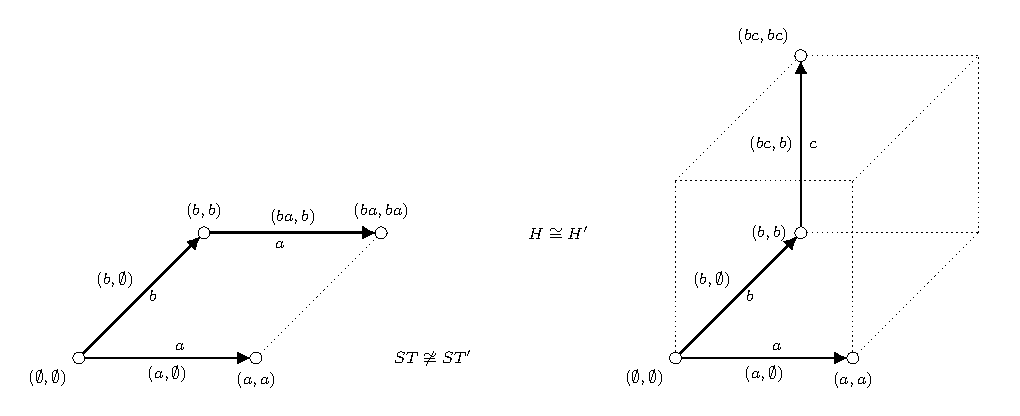
\includegraphics[scale=0.9]{Figures/4.Relationship-with-other-models-of-concurrency/ST-structure-and-HDA/Asymmetric-conflict.pdf}
            \captionof{figure}[Asymmetric conflict]{Example of ST-structures and higher-dimensional automata representing the asymmetric conflict $a + b$. The higher-dimensional automaton (left) is isomorphic to the higher-dimensional automaton (right). On the other hand, we see that the ST-structure (left) is not isomorphic to the ST-structure (right). Since, the ST-structure (left) is on two events and the ST-structure (right) is on three events.}
            \label{fig:asymmetric-conflict-st-hda}
        \end{figure}
    
        The example has no concurrency and involves two events, imposing the only restriction that once event $a$ happens, then event $b$ cannot occur anymore. 
    
        Higher-dimensional automata are not good at identifying the particular events, making the representation of the example as a higher-dimensional automaton challenging. Higher-dimensional automata are state-based models that represent events by actions, where actions are labels for the particular events. These actions may occur multiple times, where events only occur once in an execution. The standard way of identifying events in higher-dimensional is by equivalence classes of transitions, where two transitions are equivalent when they are parallel in the boundary of a filled square, see Figure \ref{fig:HDA-filled-interleaving-square}.
    
        The equivalence classes of transitions for higher-dimensional automata, shown in Figure \ref{fig:asymmetric-conflict-st-hda} (left), would not result in the corresponding 2-event ST-structure, which is what we want. However, would result in the 3-event ST-structure of Figure \ref{fig:asymmetric-conflict-st-hda} (right). The 2-event ST-structure is not isomorphic to the 3-event ST-structure. On the other hand, the two representations of the higher-dimensional automata from Figure \ref{fig:asymmetric-conflict-st-hda} (left and right) are isomorphic.
    \end{example}
    
    In \cite[Proposition 3.39]{Johansen16STstruct}, the mapping $\stintoh$ from Definition~\ref{def:ST-structures-to-HDA} preserves isomorphism. However, it may collapse non-isomorphic ST-structures into isomorphic higher-dimensional automata. Consider the two ST-structures from Figure~\ref{fig:asymmetric-conflict-st-hda} which are not isomorphic since the left one is defined by two events while the right one is defined by three events, whereas the higher-dimensional automata that the mapping $\stintoh$ associates are isomorphic. This means that $\stintoh$ is not an embedding from $\allST$ to $\allHDA$ since it looses information, namely, the events. A natural question to raise is if a mapping from $\allHDA$ to $\allST$ is then an embedding from $\allHDA$ to $\allST$. We will first define a mapping from $\allHDA$ to $\allST$.
    
    \begin{definition}[Events equivalence relation of $\HDA$ \cite{Johansen16STstruct}]
        \label{def:events-equivalence-relation-of-HDA}
        Define a relation $\eventEquivHDAs\ \subseteq \mathcal{Q}_{1}\times \mathcal{Q}_{1}$ on transitions of $\mathcal{H}$ as 
        
        \[
            q_{1}\eventEquivHDAs q_{1}' \quad\text{iff}\quad \exists q_{2}\in
            \mathcal{Q}_{2}:\alpha_{i}(q_{2})=q_{1}\wedge \beta_{i}(q_{2})=q_{1}'
        \]
        for some $i\leq 2$ and $\alpha,\beta\in\{s,t\}$.  Consider the reflexive and transitive closure of the above relation, and denote it the same. This is now an equivalence relation on $\mathcal{Q}_{1}$.
        % Consider an equivalence class $\equivClass{q_{1}}$ to be all
        % $q_{1}'$ equivalent with $q_{1}$.  Such an equivalence class is
        % called \emph{an event}.
    \end{definition}
    

    \begin{definition}[$\allHDA$ to $\allST$ \cite{Johansen16STstruct}]
        \label{def:HDA-to-ST-structure}
         Define a map $\ST:\allHDA \rightarrow \allST$ which builds an ST-structure $\ST(\mathcal{H})$ by associating to each rooted path $\pi\in \mathcal{H}$ an ST-configuration as follows.

        \begin{enumerate}
            \item\label{hintost_1} for the minimal rooted path which ends in $I$ associate $(\emptyset,\emptyset)$;
            \item\label{hintost_2} for any path $\pi$ which ends in a transition $\finishPath{\pi}=q_{1}\in \mathcal{Q}_{1}$ then 
        
            \begin{enumerate}
                \item\label{hintost_21} add the ST-configuration $\hintost(\pi)=\hintost(\pi_{s})\cup(\equivClass{q_{1}},\emptyset)$, where $\pi_{s}$ is a shorter path reaching through an s-map the homotopy class of $\pi$, that is, $\pi_{s}\transition{s}q_{1}\in\homotopyClass{\pi}$;
                \item\label{hintost_22} add the ST-configuration $\hintost(\pi\transition{t}q_{0})=\hintost(\pi)\cup(\emptyset,\equivClass{q_{1}})$;
            \end{enumerate}

            \item\label{hintost_3} for any path $\pi$ which ends in a higher cell $\finishPath{\pi}=q_{n}\in \mathcal{Q}_{n}$, with $n\geq 2$, then add the ST-configuration $\hintost(\pi)=\hintost(\pi^{i})\cup\hintost(\pi^{j})$, with $\pi^{i}\neq\pi^{j}$, $\pi^{i}\transition{s}q_{n}\in\homotopyClass{\pi}$, and $\pi^{j}\transition{s}q_{n}\in\homotopyClass{\pi}$.
        \end{enumerate}
    \end{definition}

    As shown in \cite[Proposition 3.42]{Johansen16STstruct}, the mapping $\ST$ associates an acyclic and non-degenerate higher-dimensional automata with $\ST(H)$, which is a rooted, connected, and adjacent-closed ST-structure. Furthermore, in \cite[Proposition 3.44]{Johansen16STstruct}, the mapping $\ST$ from Definition~\ref{def:HDA-to-ST-structure} preserves isomorphism of reachable parts. However, it may collapse non-isomorphic higher-dimensional automata into isomorphic ST-structures. This can be seen by considering the two higher-dimensional automata from Figure \ref{fig:Unfolding-HDA}, which are translated into the same ST-structure by $\ST$. The mapping $\ST$ considers the two higher-dimensional automata which are not isomorphic to be two ST-structures which are isomorphic. The higher-dimensional automata are not isomorphic since the right one has a split corner whereas the left one is a square with its faces nicely placed, forming a complete square. 
        
    \begin{figure}[ht]
        \centering
        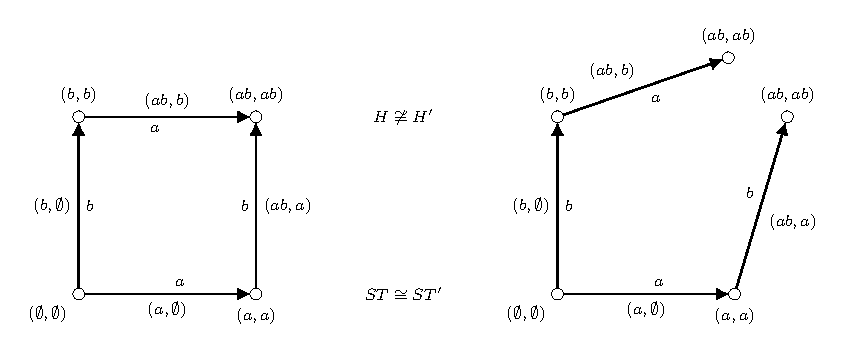
\includegraphics[scale=0.9]{Figures/4.Relationship-with-other-models-of-concurrency/ST-structure-and-HDA/HDA-collapse.pdf}
        \captionof{figure}[History unfolding of a square $\HDA$ through $\hintost$]{Example of ST-structures and higher-dimensional automata representing the unfoldings of a square $\HDA$ through $\hintost$. The ST-structure (left) is isomorphic to ST-structure (right). On the other hand, we see the higher-dimensional automaton (right) is not isomorphic to the higher-dimensional automaton (left). Since, the higher-dimensional automaton (right) has a split corner and the higher-dimensional automaton (left) is a nicely shaped square.}
        \label{fig:Unfolding-HDA}
    \end{figure}
    
    The mapping $\ST$ is not an embedding from $\allHDA$ to $\allST$ since it looses information, which in the example is the ability to announce the difference between when $a$ happens before $b$, or $b$ happens before $a$. This can also be seen, geometrically, as not being able to see the difference between the split corner of a square and a nicely shaped square.

    In Figure \ref{fig:asymmetric-conflict-st-hda}, we can see that higher-dimensional automata are not able to precisely identify events, but can be faithfully interpreted as ST-structures. ST-structures are able to precisely capture events while events in higher-dimensional automata are not easily captured. As we have shown in Figure \ref{fig:Unfolding-HDA}, ST-structures are not able to capture the difference between a higher-dimensional automaton and the unfolding of that higher-dimensional automaton. Hence, some processes might only be able to be represent as higher-dimensional automata, and identifying precisely these events of the processes would be challenging. We are interested in finding a model that is able to capture the aspect of higher-dimensional automata, but also be faithfully translated to ST-structures. In this regard, we will investigate Chu spaces and ST-structures.
\section{Chu spaces and ST-structures}
\label{sec:Chu-spaces-and-ST-structures}
    Chu spaces can be viewed in various equivalent ways, as mentioned in Section \ref{sec:Chu-spaces}. A Chu space can be viewed as a matrix with entries from $K$, where rows represent the events from $E$ and columns represent the configurations in $X$.
    
    ST-structures capture the "\emph{during}" aspect in the event-based setting, extending configuration structures with this notion. We consider Chu spaces $K= \mathbf{3}= \{0, \executing , 1\}$ with the order $0 < \executing\ < 1$, introducing the value $\executing$ to stand for \textit{during}, or \textit{in transition}. We see that Chu space over $\mathbf{3}$ is similar to the sculpting way of looking at Chu spaces as mentioned at the end of Section \ref{sec:Chu-spaces}. Hence, revealing the intrinsic symmetry of events and states. Chu space over $\mathbf{3}$ is also called a triadic chu space.


    \begin{definition}[Translations between ST and Chu]
        \label{def:ST-to-Chu}
        For an ST-structure $\ST$ over $E$ construct $\chu{E}{X}^{\ST}$ the associated Chu space over $\mathbf{3}$ with $E$ the set of events from $\ST$, and $X\subseteq \mathbf3^{E}$ containing for each ST-configuration $(\mathcal{S},\mathcal{T})$ the state $x^{(\mathcal{S},\mathcal{T})}\in X$ formed by assigning to each $e\in E$:
  
        \begin{itemize}
            \item $e \rightarrow 0$ if $e\not\in \mathcal{S}$ and $e\not\in \mathcal{T}$;
            \item $e \rightarrow \executing$ if $e\in \mathcal{S}$ and $e\not\in \mathcal{T}$;
            \item $e \rightarrow 1$ if $e\in \mathcal{S}$ and $e\in \mathcal{T}$.
        \end{itemize}
  
        The possibility that $e\notin \mathcal{S}$ and $e\in \mathcal{T}$ is dismissed by the requirement $\mathcal{T} \subseteq \mathcal{S}$ of ST-configurations.  Call this mapping $\stintochu(\mathcal{S},\mathcal{T})$ when applied to a ST-configuration and $\stintochu(\ST)$ when applied to an ST-structure.
  
        The other way, translate a Chu space $(E,X)$ into a ST-structure over $E$ with one ST-configuration $(\mathcal{S},\mathcal{T})^{x}$ for each state $x\in X$ using the inverse of the above mapping.  We use $\chuintost(x)$ for the ST-configuration obtained from the event listing $x$. For example, for an event listing $x=(1,\executing,\executing,0)$ make the ST-configuration $\chuintost(x)=(\{e_{1},e_{2},e_{3}\},\{e_{1}\})$ where the last event $e_{4}$ does not appear neither in the first nor the second set of the ST-configuration.
    \end{definition}

    \begin{proposition}[{\cite[Section 3.4]{Johansen16STstruct}}]
        \label{prop:ST-structure-Chu-over-3}
        ST-structures are isomorphic to Chu spaces over $\mathbf{3}$, such that $\chuintost(\stintochu(\ST)) \isomorphic \ST$.
        %  by virtue of the translations from Definition~\ref{def:ST-to-Chu}.
    \end{proposition}
    
    Thus, a ST-configuration can be seen as a listing/tuple with values from $\mathbf{3}$; which exact listing of the events $E$ is irrelevant once fixed.  Therefore, when we later use ST-configurations to \emph{label} cells of an \HDA, we can alternatively use the Chu spaces notation, interchangeably.

    \begin{lemma}
        For any ST-structure $\ST$ the Chu space $\stintochu(\ST)$ is \emph{extenssional}, meaning that no two states are identical, that is, $\forall x,x'.\exists e:x(e)\neq x'(e)$.
    \end{lemma}

    \begin{proof}
        In short, since ST-structures work with sets, we have that in the set of ST-configurations there are no two ST-configurations that are the same, then the states produced by $\stintochu$ would also be different by the virtue of the assignment from Definition~\ref{def:ST-to-Chu} which associates unique events valuation to a ST-configuration.

         In detail, for any $x^{(\mathcal{S},\mathcal{T})}\neq x^{(\mathcal{S}',\mathcal{T}')}$ they are created from some different $(\mathcal{S},\mathcal{T})\neq (\mathcal{S}',\mathcal{T}')$, which implies one of the two cases:
        
        \begin{enumerate}
            \item When $\mathcal{S} \neq \mathcal{S}'$ then pick some $e\in \mathcal{S}$ such  that $e\notin \mathcal{S}'$ (or the other way around if needed) then the states generated by $\stintochu$ would have the valuations: $x^{(\mathcal{S},\mathcal{T})}(e)\in\{\executing,1\}$ and $x^{(\mathcal{S}',\mathcal{T}')}(e)=0$, thus making them different.
            \item When $\mathcal{S} = \mathcal{S}'$ but $\mathcal{T} \neq \mathcal{T}'$ the pick some $e \in \mathcal{T}$ such that $e \notin \mathcal{T}'$ (or the other way around if needed) then the states would have  $x^{(\mathcal{S},\mathcal{T})}(e)=1$ (because $e \in \mathcal{T} \subseteq \mathcal{S}$) and $x^{(\mathcal{S}',\mathcal{T}')}(e) = \executing$, thus making them different.
        \end{enumerate}
    \end{proof}
    
    In Section \ref{sec:Chu-spaces}, a morphism between Chu spaces ($E, X$) and ($A, Y$) is defined to be a pair ($f, g$) of maps $f : E \to A$ and $g: Y \to X$ that satisfy the adjointness condition. We can extend $\stintochu$ to a functor between the two categories $\categoryST$ and $\categoryChu$\ by defining its application to morphisms as $\stintochu(f)=(f,g)$ with $g$ defined in terms of $f$ using the equation~\refeq{categoryChu1}.

    \begin{lemma}
        The $\stintochu$ is a functor between $\categoryST$ and $\categoryChu$.
    \end{lemma}

    \begin{proof}
        Since the Chu-spaces generated by $\stintochu$ are extensional, then we define $g$ by defining what the values of all the events are from $A$ in that state from $X$ as $g(y)(e)=y(f(e))$. This now makes the two mapings $(f,g)$ to respect the adjointness condition of the category $\categoryChu$, that is, to be a proper morphism in this category.
    \end{proof}

    Note that \chuintost\ cannot be a functor because the Chu-transforms are too weak
    % make too few relations between events of states of the two Chu-spaces
    to allow us to prove the configuration-preserving property of the ST-morphisms.
\section{Summary}
    \label{sec:traditional-concurrency-summary}

    When considering the classification of concurrency models of Winskel et al. \cite{winskel94RelationshipsConcurrency}, we have that models are either simulating concurrency, known as \emph{interleaving}, or dealing directly with concurrency, namely \emph{non-interleaving}. The difference being that mutually exclusive occurrences are not distinguishable from truly independent ones in the former, but distinguishable in the latter.
    
    Interleaving models are not able to distinguish mutually exclusive events from truly independent events because the models depend on which events a process takes to be \emph{atomic} \cite[page 4]{Pratt86pomsets}. When we say atomic, we mean an indivisible action that must complete without interruption, in other words be considered instantaneous. If we suppose that an atomic event can be \emph{refined} in the same manner as how Pratt explains refinement of atomic actions in \cite{pratt91hda}, then the interleaving model can be seen to not have interleaved subactions. We will consider such a refinement as \emph{action refinement}. Action refinement is the method of developing a system by starting from a abstract specification, and gradually refining its action by providing more details \cite{Johansen16DecEventBasedConcurrencyRefinement, GlabbeekG89refinement}.
    
    % In the literature, it has shown that interleaving models are not well behaved under action refinement. \cite{x,y,z}.
    In the literature, it has been shown that interleaving models are not well behaved under action refinement \cite{GlabbeekG89refinement, GlabbeekG01refinement}. The model is forced to commit itself in advance to a particular level of granularity. For example, a programmer may give details on actions that, at the time, are regarded as atomic. However, at a future release the programmer may discover that the actions have substructures, see \cite[Example 1.1]{GlabbeekG89refinement}. The programmer cannot refine the action since it is atomic. There might be occurrences where the interleaving model can be seen not to have interleaved subactions. The failure  to interleave subactions is not characteristic of non-interleaving concurrency, but rather of a hidden assumption of excluded middle, or \emph{mutual exclusion} as it is more commonly known in concurrent processes \cite{Pratt00Sculptures}. We consider mutual exclusion to be where no actions can happen simultaneously, and must occur after each other.
    
    From our definition of transition systems, we are only able to simulate the parallel execution of two actions as the "\emph{interleaving}" of $ab$ or $ba$, see Figure \ref{fig:transition-system}. In the next chapter we will introduce asynchronous transition systems which extends the transition system to include an independence relation that is equipped to distinguish the mutual exclusion and independent occurrence of two events.


\chapter{Sculpting in concurrency}

\label{chap:sculpting-in-concurrency}

    
    In this chapter we define a method of modelling concurrent behaviour of higher-dimensional automata. We call this method \emph{sculpting}. In other words, the process of modelling a concurrent system using higher-dimensional automata may be considered as a sculpting process $-$ take one single higher-dimensional cube, having enough concurrency, meaning enough events, and remove cells until the desired concurrent behaviour is obtained. The model obtained is called a \emph{sculpture}.
    
    We investigate the method of sculpting which has not been studied for higher-dimensional automata before. One goal is to tighten the correlation between ST-structures and higher-dimensional automata, which was left open in \cite{Johansen16STstruct} where neither model could be embedded into the other. The main result of our study is the fact that the sculpting method cannot build all higher-dimensional automata, but only a strict subset of these. We identify the category of sculptures and its relation to the category of higher-dimensional automata and the category of ST-structures.
\section{Sculptures}
\label{sec:sculptures}
    The intuition for the method of programming as sculptures was first introduced by Pratt in \cite{Pratt00Sculptures} as a method of identifying events in higher dimensional automata. It was considered in regards to the Chu space approach to higher dimensional automata, where one instead starts with a single cube of very large, possibly infinite, dimension and "\emph{sculpts}" the desired process by removing unwanted faces. Initially, a cube constitutes the events to be a discrete and unstructured set, forming a complete cube. By removing states, the event set becomes structured. For example, sculpting two events by removing all the states distinguishing them renders them equivalent. The removal of states from higher-dimensional automata may be understood as furnishing higher-dimensional automata with a certain structure.
    
    A sculpture consists of a higher-dimensional automaton, a bulk and an embedding. A \emph{bulk} is a \emph{non-selflinked} precubical set which is generated by a single cube of very large, possibly infinite, dimension. A precubical set $\mathcal{X}$ is \emph{non-selflinked} if it holds for all $x, y\in \mathcal{X}$ that there exists at most one index sequence $i_1\le\dotsc\le i_n$ such that $x= \alpha^1_{ i_1}\dotsm \alpha^n_{ i_n} y$ for $\alpha^1,\dotsc, \alpha^n\in\{ s, t\}$. Hence, there is unique representation for each cell in the precubical set. An embedding is an injective morphism such that there is a mapping from the precubical set to the bulk. Intuitively, an embedding is considered to be the same as sculpting the desired process by removing unwanted faces.

    \begin{definition}[Bulk]\label{def:bulk}
        A precubical set $\mathcal{X}$ is a \emph{bulk} if it is non-selflinked and generated by precisely one $n$-cube, that is, if $\num{ \mathcal{X}_{ \dim X}}= 1$.
    \end{definition}

    Any two $d$-dimensional bulks are isomorphic, where the isomorphism is generated by a permutation of the $d$ directions of the generating cubes.  Hence we may talk of \emph{the} $d$-dimensional bulk, and denote it by $\bulk{d}$.

    We develop a naming scheme for bulks inspired by Chu spaces. 

    \begin{definition}[Canonical naming]
    \label{def:canonical-naming}
        Fix $d\in \Nat$ and let $\bulk{d}= \{ 0, \executing, 1\}^d$. For $n= 0,\dotsc, d$, let $B_n=\{( x_1,\dotsc, x_d)\in B\mid \num{\{ i\mid x_i= \executing\}}= n\}$ be the set of tuples with precisely $n$ occurrences of $\executing$.  For $n= 1,\dotsc, d$, define face maps $s_k, t_k: B_n\to B_{ n- 1}$ ($k= 1,\dotsc, n$) as follows: for $x=( x_1,\dotsc, x_d)\in B_n$ with $x_{ i_1}=\dotsm= x_{ i_n}= \executing$, let $s_k x=( x_1,\dotsc, 0_{ i_k},\dotsc, x_d)$ and $t_k x=( x_1,\dotsc, 1_{ i_k},\dotsc, x_d)$ be the tuples with the $k$-th occurrence of $\executing$ set to $0$ or $1$, respectively. We call this the \emph{canonical naming} for the bulk $\bulk{d}$.
    \end{definition}

    The above construction essentially labels the $d$-bulk with lists of Chu-labels, namely, with states from the Chu space on $d$ events. Any cell $q^{b}$ in a bulk $\bulk{d}$ is reached from the highest cell $q_{d}$ through a sequence of face maps applications $\alpha_{i_{1}}\dotsm \alpha_{i_{k}}q_{d}=q^{b}$ of correct indices. 

    \begin{lemma}
        \label{lemma:chu-labelling-bulk}
        The structure $\bulk{d}$ as defined above is the $d$-dimensional bulk.
    \end{lemma}

    \begin{proof}
        It is trivial to check that $B$ is a precubical set.  $\bulk{d}$ is also non-selflinked, and $\num{ B_d}= \num{\{( \executing,\dotsc, \executing)\}}= 1$, thus by uniqueness up to isomorphism, $\bulk{d}$ is the $d$-dimensional bulk.
    \end{proof}

    The \emph{initial state} $\initbulk{d}$ of the bulk $\bulk{d}$ is the cell named $( 0,\dotsc, 0)$ in the canonical naming.  (any automorphism of $\bulk{d}$ fixes this cell.)  This turns bulks into $\HDA$.

    The $d$-dimensional bulk can be embedded into any bulk of dimension $d'\ge d$ by using the embedding $\embedMorphism^{d'}_{d}:\bulk{d}\hookrightarrow \bulk{d'}$ which maps any cell $( t_1,\dotsc, t_d)$ to $( t_1,\dotsc, t_d, 0,\dotsc, 0)$ in the canonical naming.  It can easily be shown that up to isomorphism, $\embedMorphism^{ d'}_d$ is the \emph{only} $\HDA$ morphism from $\bulk{ d}$ to $\bulk{ d'}$, hence also that there are no $\HDA$ morphisms $\bulk{d}\to \bulk{d'}$ for $d'< d$.

    \begin{definition}[Sculpture]
        \label{def:sculptures}
        A \emph{sculpture} is a $\HDA$ $\mathcal{X}$ together with a bulk $\bulk{d}$ and a $\HDA$ embedding morphism, in other words, an injective morphism, $\embedMorphism: X\hookrightarrow \bulk{d}$. We denote a sculpture by ($\mathcal{X}, \bulk{d}, \embedMorphism$).

        \emph{morphism} of sculptures $\embedMorphism: \mathcal{X} \hookrightarrow \bulk{ d}$, $\embedMorphism': \mathcal{X}' \hookrightarrow \bulk{ d'}$ is a pair of $\HDA$ morphisms $f: \mathcal{X} \to \mathcal{X}'$, $b: \bulk{ d}\to \bulk{ d'}$ such that the square

        \begin{equation*}
            \xymatrix{%
            \mathcal{X} \ar[d]_{\embedMorphism} \ar[r]_f & \mathcal{X}' \ar[d]^{\embedMorphism'}
            \\ \bulk{d} \ar[r]^b & \bulk{d'}
            }
        \end{equation*}

        commutes, namely, $b\circ \embedMorphism= \embedMorphism'\circ f$.  By the above considerations, this entails that $d'\ge d$ and $b$ is injective, hence also $f$ must be injective.  To sum up, morphisms of sculptures are commuting squares of embeddings. Two sculptures are isomorphic, denoted $\isomorphic$, when the morphism between them has both $f,b$ bijections; thus making the bulks of the same dimension.
    \end{definition}

    \begin{remark}
        One precubical set can be seen as two different sculptures, for example, from two different dimensional bulks, in both cases being a simplistic sculpture, meaning it all depends on the embedding morphism. Then this precubical set enters as source object of several sculpture morphisms, as seen in Figure~\ref{fig:asymmetric-conflict-st-hda}.
    \end{remark}
    
    The major problem with both translations is related to the fact that it is not clear how to identify the events in a higher-dimensional automaton. The best example for this is the fact that the mapping ST destroys the interleaving square, which is due to the fact that the standard method of identifying events in a higher-dimensional automaton by equivalent transitions opposite in a filled square fails for this unfilled square; see Figure \ref{fig:HDA-broken-box} (left). This same issue about events is also the one that causes the problem for the other mapping H where we could not say in the higher-dimensional automaton that was generated whether this was representing two or three events.
    
    However, we show how sculpting allows to identify the events in a higher-dimensional automaton in the same way as ST-structures work with events (we still use the standard intuitive method of seeing events as equivalence classes of transitions opposite in a filled square).
    
    We show that the ST-structures captures precisely the higher-dimensional automaton that can be seen as sculptures. 


\section{Sculptures and ST-structures}
    \label{sec:sculpture-and-st-structure}

    We show that sculptures and ST-structures are isomorphic while also respecting the computation steps. This result resolves the open problems noticed in \cite[Section 3.3]{Johansen16STstruct} that there is no adjoint between the two translations given there between ST-structures and higher-dimensional automata. We are using here the same translations, but add more information that is given by the bulk and the embedding of the sculpture, which allows us to obtain a one-to-one mapping between ST-structures and this class of higher-dimensional automata that sculptures form.
    
    Through the observation from Section~\ref{sec:Chu-spaces-and-ST-structures}, the results in this Section extend to Chu spaces over \textbf{3} as well. Thus, Chu spaces are not enough to capture the concurrency that general higher-dimensional automata can express.
    
    From Section \ref{sec:st-structure-and-hda}, we considered the mapping of $\allST$ into $\allHDA$ which was taken from \cite{Johansen16STstruct}. We showed that for a rooted, connected, and adjacent-closed ST-structure $\ST$ the mapping associates a higher dimensional automaton respecting all precubical identities and is acyclic and non-degenerate. Also, we showed that the order in which the events were picked did not matter.
     
    This mapping can be extended to generate a sculpture, in other words, the dimension of the sculpture and the embedding, thus retaining the information about the events from the ST-structure it encodes.

    \begin{definition}[\allST\ to sculptures]
        \label{def:ST-to-Sculptures} 
        We define a mapping $\stintosculpture$ that for any ST-structure generates an $\HDA$, as well as a bulk and an embedding, thus a sculpture, as follows.  Consider an $\ST=(E,ST)$, with the events linearly ordered as a list $\evlist{E}$. Then $\stintosculpture(\ST)$ returns the $\HDA$ which
  
        \begin{itemize}
            \item has cells $\mathcal{Q}=\{q^{(\mathcal{S},\mathcal{T})}\in \mathcal{Q}_{n} \mid (\mathcal{S},\mathcal{T})\in ST \mbox{ and } \num{(\mathcal{S} \setminus \mathcal{T})}=n\}$;
            \item for any two cells $q^{(\mathcal{S},\mathcal{T})}$ and $q^{(\mathcal{S} \setminus e,\mathcal{T})}$ add the map entry $s_{i}(q^{(\mathcal{S},\mathcal{T})})=q^{(\mathcal{S} \setminus e,\mathcal{T})}$ where $i$ is the index of the event $e$ in the listing $\evlist{E}\!\!\downarrow_{(\mathcal{S} \setminus \mathcal{T})}$;
            \item for any two cells $q^{(\mathcal{S},\mathcal{T})}$ and $q^{(\mathcal{S},\mathcal{T} \cup e)}$ add the map entry $t_{i}(q^{(\mathcal{S},\mathcal{T})})=q^{(\mathcal{S},\mathcal{T} \cup e)}$ where $i$ is the index of the event $e$ in the listing $\evlist{E}\!\!\downarrow_{(\mathcal{S} \setminus \mathcal{T})}$.
        \end{itemize}
        
        $\evlist{E}\!\!\downarrow_{(\mathcal{S} \setminus \mathcal{T})}$ is the listing $\evlist{E}$ restricted to the set $\mathcal{S} \setminus \mathcal{T}$.
 
        Build the bulk $\bulk{n}$, with $n=\num{(E)}$, as in Lemma~\ref{lemma:chu-labelling-bulk} using the canonical naming on the same listing of the events $\evlist{E}$ as used to generate the above $\HDA$.  The embedding $\embedMorphism:\stintosculpture(\ST)\hookrightarrow \bulk{n}$ is defined as $\embedMorphism(q^{(\mathcal{S},\mathcal{T})})=\stintochu(\mathcal{S},\mathcal{T})$ returning the Chu-labelling as in Proposition~\ref{prop:ST-structure-Chu-over-3} on the same listing of events $\evlist{E}$.
    \end{definition}
    
    The mapping $\stintosculpture$ translates a rooted, connected, and adjacent-closed ST-structure $\ST$ into a higher dimensional automaton, respecting all cubical laws. Moreover, it is immaterial which listing of the events is picked in the definition (these results are direct adaptations of results from \cite{Johansen16STstruct}). This mapping preserves isomorphism of ST-structures, and moreover, it does not collapse non-isomorphic ST-structures.

    \begin{proposition}
        \label{prop:ST-to-Sculpture-iso}
         For ST-structures $\ST$ and $\ST'$, $\ST\isomorphic \ST'$ iff\/ $\stintosculpture(\ST)\isomorphic\stintosculpture(\ST')$
    \end{proposition}

    \begin{proof}
         It is clear that $\ST\isomorphic \ST'$ implies $\stintosculpture(\ST)\isomorphic\stintosculpture(\ST')$.  We now show that $\stintosculpture(\ST)\isomorphic\stintosculpture(\ST')$ implies $\ST\isomorphic\ST'$. We show the existence of an isomorphism over the ST-structures, knowing the isomorphism over their translations as sculptures, making use of a fixed listing of events that the map \stintosculpture\ works with, the same listing for both translations, since we know the translation can choose any listing.
        % The rest is tedious details.

        Since the two sculptures $\stintosculpture(\ST)\isomorphic\stintosculpture(\ST')$ are isomorphic it means that the $\HDA$s are embedded in the same bulk, which means we are working with the same set of events $E=E'$ generated by \stintosculpture, modulo a reordering of their listing, which is captured by the second map $b$ between the bulks. We know that $b$ is a bijection on the cells of the bulks, and thus, through the canonical naming scheme, $b$ induces a bijection on $E$ which we call $g$ defined by $g(e_{i})=e'_{i}$ where the index $i$ is important (i.e., $g$ associates the event on position $i$ in the listing $\evlist{E}$ with the event on the same position in the listing $\evlist{E'}$). We use $g$ as the isomorphism that we are looking for between the two ST-structures. 

        We need to show that $g$ preserves configurations, i.e., for some $(\mathcal{S},\mathcal{T})\in\ST$ we prove that $g(\mathcal{S},\mathcal{T}) \in \ST'$. We make use of the commuting square property of the sculpture morphisms. For the ST-configuration there exists the corresponding cell $q^{(\mathcal{S}, \mathcal{T})}$ generated by the \stintosculpture, which in turn is embedded in the bulk as $\stintochu(\mathcal{S},\mathcal{T})$. At the same time the HDA morphism associates $f(q^{(\mathcal{S},\mathcal{T})})=q^{(\mathcal{S}',\mathcal{T}')}$ to some cell in $\stintosculpture(\ST')$ which in turn comes from some ST-configuration $(\mathcal{S}',\mathcal{T}')$. This cell is embedded into the bulk as $\stintochu(\mathcal{S}',\mathcal{T}')$ which is equated to $\stintochu(\mathcal{S},\mathcal{T})=b(\stintochu(\mathcal{S},\mathcal{T}))$ by the bulk isomorphism, meaning that respective events in the two listings receive the same values. Now, going through the translation between Chu states and ST-configurations we can see how $g(\mathcal{S},\mathcal{T})=(g(\mathcal{S}),g(\mathcal{T}))=(\mathcal{S}',\mathcal{T}')\in\ST'$.

        \begin{itemize}
            \item If $e_{i} \not\in \mathcal{S}$ then $\stintochu(\mathcal{S},\mathcal{T})(e_{i})=0$, which means that also $g(e_{i})=e'_{i}$ takes the same value in $\stintochu(\mathcal{S}',\mathcal{T}')(g(e_{i}))=0$. This means that $g(e_{i})\not\in \mathcal{S}'=g(\mathcal{S})$ because of injectivity.
            \item If $e_{i}\in \mathcal{S}$ and $e_{i} \not\in \mathcal{T}$ then $\stintochu(\mathcal{S},\mathcal{T})(e_{i})=\executing$, which means that also $g(e_{i})=e'_{i}$ takes the same value in $\stintochu(\mathcal{S}',\mathcal{T}')(g(e_{i}))=\executing$. This means that $g(e_{i})\in g(\mathcal{S})$ and $g(e_{i}) \not\in g(\mathcal{T})$ because of injectivity on $\mathcal{S}$.
            \item If $e_{i}\in \mathcal{T} \subseteq \mathcal{S}$ then $\stintochu(\mathcal{S},\mathcal{T})(e_{i})=1$ which means that also $g(e_{i})=e'_{i}$ takes the same value in $\stintochu(\mathcal{S}',\mathcal{T}')(g(e_{i}))=1$. This means that $g(e_{i}) \in g(\mathcal{T}) \subseteq g(\mathcal{S})$.
        \end{itemize}
    
        This proves that $(g(\mathcal{S}),g(\mathcal{T}))\in\ST'$.
    
    \end{proof}

    \begin{definition}[Sculptures to $\allST$]
        \label{def:sculptures-to-ST}
        Define a mapping $\sculpintost$, which for a sculpture $\sculpture{\mathcal{H}}{n}=(\mathcal{H},\bulk{n},\embedMorphism)$ associates the ST-structure $\sculpintost(\sculpture{\mathcal{H}}{n})$ as follows. Take a linearly ordered set $\evlist{E}$ (of events) of cardinality as the dimension of the bulk $n=\dim\bulk{n}$. The ST-configurations of $\sculpintost(\sculpture{\mathcal{H}}{n})$ are obtained from the cells of $H$ as $\sts=\{\chuintost(\embedMorphism(q)) \mid q\in \mathcal{H}\}$.
    
    \end{definition}

    Intuitively, since we have the bulk we can work with the canonical naming based on a fixed listing of events. Using Proposition~\ref{prop:ST-structure-Chu-over-3} we can associate an ST-configuration to each cell of the $\HDA$ by going through the embedding to the corresponding cell in the bulk. It is clear that $\sculpintost(\sculpture{\mathcal{H}}{n})$ is rooted, connected and closed under single events, that is, regular.

    The following results show a one-to-one correspondence between the ST-structures and sculptures.

    \begin{proposition}
        \label{prop:ST-to-Sculpture}
        For an arbitrary ST-structure $\ST$ we have
        \[
            \sculpintost(\stintosculpture(\ST))\isomorphic \ST.
        \]
    \end{proposition}

    \begin{proof}
        To prove the isomorphism between the right-hand $\ST=(E,\sts)$ and the left-hand $\sculpintost(\stintosculpture(\ST))$ we need to show that $\exists f: E \parto E'$ such that $f$ preserves ST-configurations.  
        % and is locally injective and total, 
        % i.e., for all $( S, T)\in \sts$ we show that $f( S, T):=( f( S), f( T))\in \sts'$, with $\sts'$ the ST-configurations generated on the left-hand side.
        %  and for all $( S, T)\in \sts$, the restriction $f\rest S$ is injective and total). 
        We will consider $E'$ to be the events produced by the left-hand side of the isomorphism, precisely, by $\sculpintost(\stintosculpture(\ST))$.
    
        The application of the mapping $\stintosculpture$ 
        % provided in Definition \ref{def_stintosculptures} which 
        generates an $\HDA$, as well as a bulk and an embedding, considering the events of $\ST$ to be linearly ordered as a list $\evlist{E}$. $\stintosculpture$ builds cells $\mathcal{Q}=\{q^{(\mathcal{S},\mathcal{T})}\in \mathcal{Q}_{n} \mid (\mathcal{S},\mathcal{T})\in\sts \mbox{ and } \num{(\mathcal{S} \setminus \mathcal{T})}=n\}$ and the embedding $\embedMorphism(q^{(\mathcal{S},\mathcal{T})})=\stintochu(\mathcal{S},\mathcal{T})$ into the bulk $\bulk{\num E}$; thus the sculpture $\sculpture{\mathcal{H}}{n}=(\mathcal{Q}, \bulk{\num E}, \embedMorphism(q^{(\mathcal{S},\mathcal{T})}))$. The embedding $\embedMorphism$ returns for each cell $q^{(\mathcal{S}, \mathcal{T})}$ the Chu-labelling as in Proposition~\ref{prop:ST-structure-Chu-over-3} on the same listing of events $\evlist{E}$.
   
        Thus, the ST-structure produced on the left-hand side by $\sculpintost$ applied to the above sculpture $\sculpture{\mathcal{H}}{s}(\ST)=\sculpture{\mathcal{H}}{n}$ assumes, without loss of generality, to have the same listing of events $\evlist{E}$ as before.
        % , i.e., as produced by \sculpintost\ according to Definition~\ref{def_sculptures_to_ST}.
        % 
        The ST-configurations of $\sculpintost(\sculpture{\mathcal{H}}{n})$ are obtained from the cells of $\sculpture{\mathcal{H}}{n}$ as $\sts' = \{\chuintost(\embedMorphism(q^{(\mathcal{S},\mathcal{T})})) \mid q^{(\mathcal{S},\mathcal{T})} \in \sculpture{\mathcal{H}}{n}\}$, see Definition \ref{def:sculptures-to-ST}. 

        Since $E'$ is the same set of events $E$, we take the isomorphism map $f: E \rightarrow E$ to be identity function on $E$.
        %, i.e., $\forall e\in E: f(e)=e$.
        % We show that the isomorphism properties hold. 
        We check that $f$ preserves the ST-configurations, such that $f(\mathcal{S}, \mathcal{T}):=( f(\mathcal{S}), f(\mathcal{T})) = (\mathcal{S}, \mathcal{T}) \in \sts'$. From this it must be that $\exists q^{(\mathcal{S},\mathcal{T})}\in\sculpture{\mathcal{H}}{n}: \chuintost(\embedMorphism(q^{(\mathcal{S},\mathcal{T})}) = (\mathcal{S},\mathcal{T})$ by Definition \ref{def:sculptures-to-ST}. Further, from Definition~\ref{def:ST-to-Sculptures} we know that $\chuintost(\embedMorphism(q^{(\mathcal{S},\mathcal{T})}) = \chuintost(\stintochu(\mathcal{S},\mathcal{T}))$. Finally, by Proposition \ref{prop:ST-structure-Chu-over-3} we have the expected result $\chuintost(\embedMorphism(q^{(\mathcal{S},\mathcal{T})}) = \chuintost(\stintochu(\mathcal{S},\mathcal{T})) = (\mathcal{S},\mathcal{T})$.

        It is easy to see that $f$, as identity function, is locally injective and total.
    \end{proof}

    \begin{proposition}
        \label{prop:Sculpture-to-ST}
        For any sculpture $\sculpture{\mathcal{H}}{n}=(\mathcal{H},\bulk{n},\embedMorphism)$ we have
        \[
            \stintosculpture(\sculpintost(\sculpture{\mathcal{H}}{n})) \isomorphic \sculpture{\mathcal{H}}{n}.
        \]
    \end{proposition}

    \begin{proof}
        To prove the isomorphism between the right-hand $\mathcal{H}^{n}=(\mathcal{H},B^{n}, em)$ and the left-hand $\stintosculpture(\sculpintost(\mathcal{H}^{n}))$ we need to show that $\exists f: \mathcal{H} \rightarrow \mathcal{H}'$ and $\exists b:B^{n} \rightarrow B^{n}$ such that $f,b$ are bijective and the square commutes, namely, $b \circ em = em' \circ f$.
    
        \begin{equation*}
            \xymatrix{%
            \mathcal{H} \ar[d]_{\embedMorphism} \ar[r]_f & \mathcal{H}' \ar[d]^{\embedMorphism'}
            \\ \bulk{n} \ar[r]^b & \bulk{n'}
            }
        \end{equation*}

        First, we consider the mapping $\sculpintost$ provided in Definition \ref{def:sculptures-to-ST} which generates an $ST$ for a sculpture, as follows. Take a linearly ordered set $\evlist{E}$ (of events) of cardinality as the dimension of the bulk, that is, $|E| = n = \dim \bulk{n}.$ The ST-configurations of $\sculpintost(\mathcal{H}^{n})$ are obtained from the cells of $\mathcal{H}$, such that $\forall q \in \mathcal{H} :\sculpintost(q)=STChu(\embedMorphism(q))=(\mathcal{S},\mathcal{T})^{q}$. This is the ST-structure produced on the left-hand side by $\sculpintost$ applied to the sculpture $\mathcal{H}^{n}$. 

        We will now consider the mapping $\stintosculpture$ provided in Definition \ref{def:ST-to-Sculptures} which generates a $\HDA$ for any ST-structure, as well as a bulk and an embedding, thus a sculpture, as follows. $\stintosculpture$ requires the events of the ST-structure to be linearly ordered. We take the same order produced above by $\sculpintost$.
    
        \begin{enumerate}
            \item Build the bulk $B^{n'}$, with $n'=\num E=n$, as in Lemma \ref{lemma:chu-labelling-bulk} using the canonical naming on the listing of the events $\evlist{E}$. This is thus the same bulk $\bulk{n}$ from $\mathcal{H}^{n}$. Thus we can take the $b$ part of the sculptures morphism to be the identity function which is thus a morphism between \HDA. This is also a bijection.
        
            \item The HDA $\stintosculpture(\sculpintost(\mathcal{H}^{n}))$ has cells $\mathcal{Q}=\{p^{(\mathcal{S},\mathcal{T})} \in \mathcal{Q}_{n} \mid (\mathcal{S},\mathcal{T}) \in \sculpintost(\mathcal{H}^{n})$ and $\num{(\mathcal{S} \setminus \mathcal{T})}=n\}$. Since each ST-configuration corresponds to some $q \in \mathcal{H}^{n}$ we thus construct one cell $p^{(\mathcal{S},\mathcal{T})^{q}}$ for each cell $q$; which according to Definition~\ref{def:sculptures-to-ST} is built using the embedding, in other words, $p^{(\mathcal{S}, \mathcal{T})^{q}} = p^{\chuintost(\embedMorphism(q))}$.
            
            \item The embedding $\embedMorphism':\stintosculpture(\sculpintost(\mathcal{H}^{n})) \hookrightarrow B^{n'}$ is defined as $\embedMorphism'(p^{(\mathcal{S},\mathcal{T})}) = Chu(\mathcal{S},\mathcal{T})$ returning the Chu-labelling as in Proposition \ref{prop:ST-structure-Chu-over-3} on the same listing of events $\evlist{E}$.
            
            We thus take $f: \mathcal{H} \rightarrow \stintosculpture(\sculpintost(\sculpture{\mathcal{H}}{n}))$ to be defined as $f(q)=p^{\chuintost(\embedMorphism(q))}$ and $f^{-1}(p^{\chuintost(\embedMorphism(q))})=q$; thus obtaining a bijection between the cells of the respective $\HDA$s.
            
            We show that $f$ is a morphism of $\HDA$s. We thus show that $f$ commutes with the face maps, such that for any $q$ we show $s_{i}(f(q))=f(s_{i}(q))$. We have $s_{i}(f(q)) = s_{i}(p^{\chuintost(\embedMorphism(q))})=s_{i}(p^{(\mathcal{S},\mathcal{T})})$ if we call $\chuintost(\embedMorphism(q))=(\mathcal{S},\mathcal{T})$. Definition \ref{def:ST-to-Sculptures} relates this $i$-th map to a cell made from the ST-configuration $(\mathcal{S} \setminus e,\mathcal{T})$ with $e$ being the $i$-th event in the listing $\evlist{E}\restrictedToSet{\mathcal{S}\setminus \mathcal{T}}$. Since the bulk uses the same listing, we thus have this ST-configuration obtained as $\chuintost(\embedMorphism(s_{i}(q)))$. On the right-hand side of the equality we have the same by definition $f(s_{i}(q))=p^{\chuintost(\embedMorphism(s_{i}(q)))}$.

            We show that the sculptures morphism square commutes. The fact that $f,b$ are bijections finishes the proof, which proves the isomorphism property. We show that $\embedMorphism(q)=\embedMorphism'(f(q))$ by working with the right-hand side: $\embedMorphism'(f(q))=\embedMorphism'(p^{\chuintost(\embedMorphism(q))})=\stintochu(\chuintost(\embedMorphism(q)))=\embedMorphism(q)$.
        \end{enumerate}    
    \end{proof}
    
    We can also understand $\sculpintost$ as labelling every cell of the sculpture with a ST-configuration, or equivalently (because of Proposition~\ref{prop:ST-structure-Chu-over-3}) with a Chu-3 state, which in the terminology of Lemma~\ref{lemma:chu-labelling-bulk} we call this a Chu-listing or Chu-label. Corollary~\ref{cor:unqiue-chu-label-in-bulk} says that this labelling is unique. Thus, in sculptures we have a one-to-one correspondence between HDA states, ST-configurations, and Chu-3 states.

    \begin{corollary}\label{cor:unqiue-chu-label-in-bulk}
        In a bulk every cell has a unique label (either as a ST-configuration or as a Chu-label representation). Thus, there are no two cells of the bulk with the same label.
    \end{corollary}

    \begin{proof}
        This is easy to see from the proofs above.
        % \cj{Do we need more detailed proof here?}
    \end{proof}
\section{Sculptures and HDA}

    The above mappings do not provide us with a procedure for deciding whether an higher-dimensional automaton, even finite, is a sculpture, because the bulk can be of any dimension, hence there are infinitely many embeddings to check. There is an alternative way of translating higher-dimensional automata into ST-structures that work on paths starting from the shortest path in the initial cell, essentially unfolding the higher-dimensional automaton.
    % This method is essentially the one used in \cite[Def.3.39]{Johansen16STstruct}, with a few simplifications and greater care taken for the notion of equivalence of events, which is essential for our purposes here.

    \begin{definition}[$\allHDA$ to $\allST$ through paths]
        \label{def:HDA-to-ST-paths}
        Define a map $\hintost:\allHDA\rightarrow\allST$ which builds a ST-structure $\hintost(\mathcal{H})$ by associating to each rooted path $\pi\in \mathcal{H}$ an ST-configuration as follows.
        \begin{enumerate}
            \item\label{hintost_1_1} for the minimal rooted path, which ends in $\mathcal{I}$, associate $(\emptyset,\emptyset)$;

            \item\label{hintost_2_2} for any path $\pi=\pi_{s}\transition{s}q_{1}$ that ends in a transition $\finishPath{\pi}=q_{1}\in \mathcal{Q}_{1}$ then 
            \begin{enumerate}
                \item\label{hintost_2_21} add the ST-configuration $\hintost(\pi)=\hintost(\pi_{s})\cup(q_{1},\emptyset)$;
                \item\label{hintost_2_22} add the ST-configuration $\hintost(\pi\transition{t}q_{0})=\hintost(\pi)\cup(\emptyset,q_{1})$;
            \end{enumerate}

            \item\label{hintost_3_3} for any path $\pi$ that ends in a higher cell $\finishPath{\pi}=q_{n}\in \mathcal{Q}_{n}$, with $n\geq 2$, then add the ST-configuration $\hintost(\pi)=\hintost(\pi^{i}) \cup \hintost(\pi^{j})$, with $\pi^{i} \neq \pi^{j}$, $\pi^{i}\transition{s}q_{n}$, and $\pi^{j}\transition{s}q_{n}$.
        \end{enumerate}
 
    \end{definition}
    
    Note that in the case~\ref{hintost_3_3} above the paths $\pi^{i},\pi^{j}$ always exist because we work with non-selflinked $\HDA$s. 
    %The same goes for the path $\pi_{s}$ used in \ref{hintost_2_21}.
    All cells are reachable through the paths considered in the above definition when applied inductively on the length of the distance from the initial cell.
    
    For every transition we add one new event to the ST-structure. This adds too many events and does not capture the geometrical intuitions about concurrency, where transitions parallel in the sides of a filled square should represent the same event. Indeed, the construction is similar to an \emph{unfolding}~\cite{Fahrenberg15PartialHDA}, except that no homotopy equivalence is applied. See~\cite[Def.~3.39]{Johansen16STstruct} for a related construction.
    
    If we are faced with an HDA which may or may not be a sculpture, then there is a minimal equivalence on its transition cells, which is exactly the equivalence of two cells appearing as opposite faces of a square, and the transitive closure. This equivalence has already been given in Definition \ref{def:events-equivalence-relation-of-HDA}. We will use the \emph{events equivalence relation} to decide if a HDA may or may not be a sculpture. The construction from Definition \ref{def:HDA-to-ST-paths} labels each \emph{cell} with one or more ST-configurations as follows:
    
    \begin{definition}
        For an HDA $H$, and using the notation of Definition~\ref{def:HDA-to-ST-paths}, let $\rho_0\subseteq H\times \hintost(H)$ be the relation given by $\rho_0=\{( q, \hintost( \pi))\mid \finishPath{\pi}= q\}$.  For an equivalence relation $\mathord\sim\subseteq Q_1\times Q_1$, let
        
        \begin{equation*}
            \rho_\sim=\{( q, \quotientofwrt{( S, T)}{\sim})\mid( q,( S, T)) \in \rho_0\}\,.
        \end{equation*}
    \end{definition}
    
    We will apply the minimal equivalence, $\eventEquivHDAs$, on the cell naming as $\rho_{\eventEquivHDAs}$.
    We use $\rho_{\eventEquivHDAs}$ to prove in Theorem~\ref{th:non-sculpting} that the HDA from Example~\ref{exp:hda-broken-box} cannot be sculpted.

    \begin{example}[Broken box example]\label{exp:hda-broken-box}
        This example is taken from \cite[Section 9.2.1]{Glabbeek06HDA}, and also found illustrated in \cite[Figure 6]{Johansen16STstruct}. As part of van Glabbeek's presentation at EXPRESS 2004, the process displayed in Figure \ref{fig:HDA-broken-box} (left) was demonstrated with the help of the audience. We name the Figure \ref{fig:HDA-broken-box} (left) for the broken box since it represent a higher-dimensional automaton which looks almost like a complete cube, but with a single corner split.
    
        \begin{figure}[ht]
            \centering
            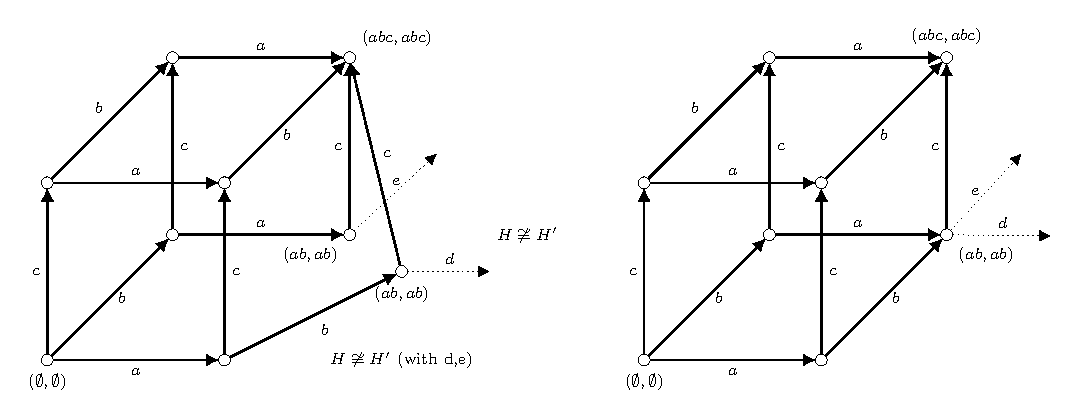
\includegraphics[scale=0.9]{Figures/5.Relationship-with-other-models-of-true-concurrency/broken_box(figure_6_left)/HDA-broken-box.pdf}
            \captionof{figure}[Broken box]{Example of sculptures, with ST-configurations as labels, and higher-dimensional automata representing the broken box example. The higher-dimensional automata (left) is not a sculpture, while the higher-dimensional automata (right) is a sculpture. We also see the higher-dimensional automaton (left) is not isomorphic to the higher-dimensional automaton (right). Since, the higher-dimensional automaton (left) has a split corner and the higher-dimensional automaton (right) is a nicely shaped cube.}
            \label{fig:HDA-broken-box}
        \end{figure}
    
        The example was of two computer scientists $A$ and $B$ travelling from one end of the podium to the other. Their task was to perform the actions $a$ and $b$, respectively, of crossing a line on the podium. Due to strategic placing of obstacles, the only place where this was possible was at a narrow opening between the obstacles that had room for only one of the scientist $A$ and $B$ at a time. This made the action $a$ and $b$ mutually exclusive, in the sense that they could not occur simultaneously.
    
        A third computer scientist $C$, was assigned the task $c$ of removing an obstacle that caused the bottleneck to exist. The action $c$ was executed causally independent of $a$ and $b$, that is, a and b are concurrent. The actions $a$ and $b$ were mutually exclusive only until $c$ occurred, after which they became causally independent.
    
        Finally, a fourth participant was assigned the task of making a statement when $a$ and $b$ had both occurred before the action $c$ started. This statement was going to be $d$ in case $A$ passed the bottleneck before $B$ did, and $e$ in case $B$ passed the bottleneck before $A$ did. Hearing this statement would prevent computer scientist $C$ from carrying out action $c$.
    
        The higher-dimensional automata (left) is not a sculpture, while the higher-dimensional automata (right) is a sculpture. We also see the higher-dimensional automaton (left) is not isomorphic to the higher-dimensional automaton (right). Since, the higher-dimensional automaton (left) has a split corner and the higher-dimensional automaton (right) is a nicely shaped cube.
    \end{example}
    
    \begin{theorem}[A non-sculpture]
        \label{th:non-sculpting}
        The $\HDA$ from Example \ref{exp:hda-broken-box} is not a sculpture.
    \end{theorem}
    
    \begin{proof}
    To show that the broken box cannot be sculpted we apply the labelling strategy described above.
    First we apply the unfolding procedure \hintost\ and for the two problematic corner states $q_{0}^{1}$ and $q_{0}^{2}$ we obtain the following ST-configurations $\hintost(\pi_{1})=(\{q_{1}^{1},q_{1}^{4}\},\{q_{1}^{1},q_{1}^{4}\})$ respectively $\hintost(\pi_{2})=(\{q_{1}^{2},q_{1}^{3}\},\{q_{1}^{2},q_{1}^{3}\})$, where $\pi_{1}$ is the lower rooted path ending in $q_{0}^{1}$ and $\pi_{2}$ is the other lower path ending in $q_{0}^{2}$.
    
    The second step is to apply the minimal equivalence \eventEquivHDAs, since this is required for any HDA. Indeed, if a HDA can be sculpted, then any cell of higher concurrency would be mapped to a unique cell in the bulk; in particular, each square from the HDA is mapped to a square in the bulk. Since we identify events in the bulk as opposite sides of bulk squares, then in the HDA any transitions opposite in a square would need to also be considered equivalent (this is what the minimal equivalence is doing).
    
    Now applying \eventEquivHDAs\ on our example equates $q_{1}^{1}\eventEquivHDAs q_{1}^{3}$ because of the three squares, front, top, back, which share the sides labelled with $a$ in the figure. (Transitivity of the equivalence was applied.)
    The same argument equates $q_{1}^{2}\eventEquivHDAs q_{1}^{4}$, this time going through the squares left-side, top, right-side.
    
    We now see that through $\rho_{\eventEquivHDAs}$ we have labelled both $q_{0}^{1}$ and $q_{0}^{2}$ with the same label $(\{[q_{1}^{2}],[q_{1}^{3}]\},\{[q_{1}^{2}],[q_{1}^{3}]\})$, made of equivalence classes.
    
    However, for a sculpture we cannot have two cells labelled the same. If an HDA can be sculpted, then we can find an embedding into a bulk. The embedding is by definition injective, meaning it maps two different HDA cells into two different bulk cells. But in the bulk each cell has a unique name in the canonical naming, as either a Chu-label or as an ST-configuration.
    \end{proof}
    
    There are more examples of non-sculptures, such as Figure \ref{fig:Unfolding-HDA}. The figure is also not representable as ST-structures and is not a sculpture. Both this example and Example~\ref{exp:hda-broken-box} are HDAs which are also their own unfoldings.


\chapter{Conclusion}
    Sculptures have been precisely defined, by following the intuition of Pratt, as well as shown to be in close correspondence with ST-structures and Chu spaces. This nicely captures Pratt's event-state-duality.
    
    We have developed an algorithm to decide whether a higher-dimensional automaton is a sculpture, and it has been used to show that, unexpectedly, some quite simple acyclic higher-dimensional automata are not sculptures. In Theorem \ref{th:non-sculpting}, we showed that a higher-dimensional automata is a sculptures, however, its unfolding is not a sculpture. We believe that this contradicts Pratt's intuition that sculptures suffice for modelling of concurrent behaviour. We may present the results of this thesis by the diagram below:
    
    \begin{center}
        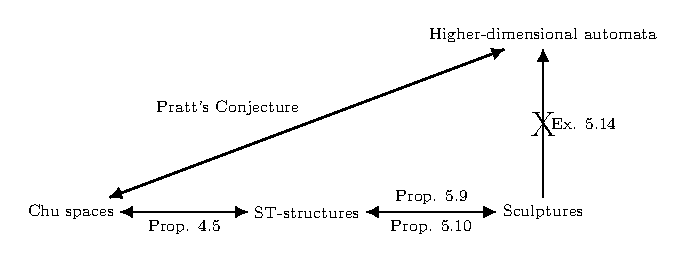
\includegraphics[scale=1]{Figures/4.Relationship-with-other-models-of-concurrency/Chu-spaces-and-ST-structures/argument-diagram.pdf}
    \end{center}
    
    In Proposition \ref{prop:ST-structure-Chu-over-3}, we showed the isomorphism between Chu spaces and ST-structures. In Proposition \ref{prop:ST-to-Sculpture} and Proposition \ref{prop:Sculpture-to-ST}, we show that ST-structures and sculptures are isomorphic. Hence, sculptures are also isomorphic to Chu spaces. To strengthen the proofs, we provided examples of higher-dimensional automata which are not sculptures, see Example \ref{exp:hda-broken-box}. We used this example to show the \emph{non-sculpting} theorem.
    
\section*{Future work}
    In this thesis, we presented combinatorial sculpting and is not to be confused with \emph{geometric} sculpting which consists of taking a geometric cube of some dimension and chiseling away hypercubes which one does not want to be part of the structure.
    
    Geometric sculpting has been used by Fajstrup et al. in~\cite{Fajstrup06AlgebraicTopologyConcurrency, Fajstrup98detectingdeadlocks, Fajstrup16DirectedAlgebraicTopologyConcurrency} and other papers to model and analyze so-called PV programs: processes which interact by locking and releasing shared resources.  In the simplest case of linear processes without choice or iteration this defines a hypercube with \emph{forbidden hyperrectangles}, which cannot be accessed due to resources access limits.  See Fig.~\ref{fig:swiss} for an example.
    
    \begin{figure}[ht]
        \centering
        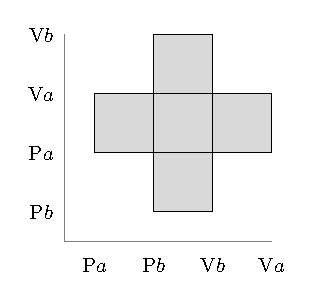
\includegraphics[scale=1.2]{Figures/6.Conclusion/swiss.pdf}
        \captionof{figure}[Swiss flag]{Two PV processes sharing two mutexes.  The forbidden area is
    grayed out.}
        \label{fig:swiss}
    \end{figure}
    
    Technically, geometric sculptures are \emph{Euclidean cubical complexes}; rewriting a proof in \cite{Ziemianski17} will show that such complexes are precisely (combinatorial) sculptures. This will be presented in a current paper, which is being submitted to FOSSACS 2019. Hence, higher-dimensional automata is Euclidean iff it is a sculpture, so that the geometric models for concurrency~\cite{Fajstrup06AlgebraicTopologyConcurrency, Fajstrup98detectingdeadlocks, Fajstrup16DirectedAlgebraicTopologyConcurrency} will show to be closely related to the combinatorial ones~\cite{pratt91hda, Glabbeek91BismiluationHDA}, through the notion of sculptures. Much work has been done in the \emph{geometric} analysis of Euclidea higher-dimensional automata~\cite{FajstrupRGH04FundCatI, GoubaultH07FundCatII, Fajstrup98detectingdeadlocks, MeshulamR17, RaussenZ14, Ziemianski17}; by the equivalences of the current work being done in the FOSSACS paper, these results will be made available for combinatorial models.
    
    As we briefly introduced in Section \ref{sec:higher-dimensional-automata}, the notion of \emph{unfolding} 
    % is important in relation to sculpting.
    % Unfolding 
    removes iteration and is commonly used to turn a complicated model into a simpler, but potentially infinite one.
    % %  (e.g., operational finite state automata vs.\ denotational event-based models). 
    % It is thus, perhaps, expected that there are simple HDA which cannot be sculpted,
    % but their unfoldings can, see Fig.~\ref{fig:unfoldings} for two examples.
    It is thus expected that even if a higher-dimensional automata cannot be sculpted, its unfolding can, as illustrated by the two simple examples in Fig.~\ref{fig:unfoldings}.
    
    \begin{figure}[tbp]
        \centering
        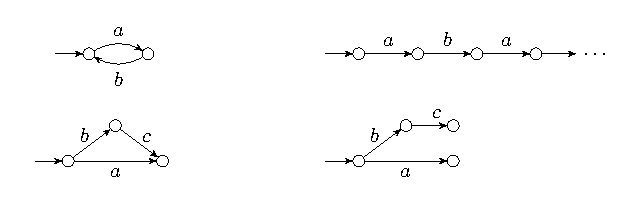
\includegraphics[scale=1.2]{Figures/6.Conclusion/unfolding.pdf}
        \captionof{figure}[Unfolding of two simple HDA]{Two simple HDA which cannot be sculpted (left) and their unfoldings (right) which can.  (The top-right sculpture is infinite.)}
        \label{fig:unfoldings}
    \end{figure}
    
    However, it can be shown that this is not the case, as witnessed by the example in Figure \ref{fig:speedAngelDemon}  which shows a higher-dimensional automaton which cannot be sculpted and which is its own unfolding. This example features two agents, $a$ and $d$, which compete to choose between two future events $b$ and $c$.  If the demon finishes his $d$ event first, then 
    % he imposes his choice between $b$ and $c$ (which he already has made before executing his $d$ event); 
    the choice between $b$ and $c$ is a demonic choice, that is, already made when starting the $d$ event;  if the angel finishes her $a$ event first, then 
    % she can freely choose between $b$ and $c$. 
    we have an instance of an angelic choice between $b$ and $c$. This system, introduced in~\cite{Johansen16STstruct}, cannot be modeled as a ST-structure, but \emph{can} be modeled as a ST-structure with \emph{cancellation}~\cite[Section~5]{Johansen16STstruct}.
    
    \begin{figure}[tbp]
        \centering
        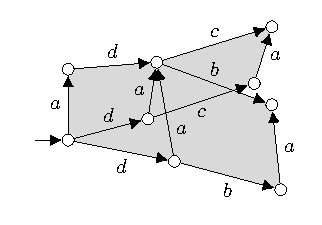
\includegraphics[scale=1.2]{Figures/6.Conclusion/angelicvsdemonic.pdf}
        \captionof{figure}[Speed game of "angelic vs. demonic choice"]{The HDA from~\cite{Johansen16STstruct} of the "speed game of angelic vs.\ demonic choice".}
        \label{fig:speedAngelDemon}
    \end{figure}

    Even more worrying is the fact that there are (acyclic) HDA which can be sculpted, but their unfoldings cannot; in fact Figure ~\ref{fig:HDA-broken-box}, is one such example. We showed, in Theorem \ref{th:non-sculpting}, that the unfolding did not return a simpler model, and which seems to contradict Pratt's claim that sculpting suffices for modeling.
    
    In the geometric setting, it can be shown that there are Euclidean cubical complexes whose unfoldings are not Euclidean.  Since Goubault-Jensen's seminal paper~\cite{Goubault92homologyof}, \emph{directed topology} (or \emph{ditopology}) has been developed in order to analyze concurrent systems as geometric objects~\cite{Grandis09book, Fajstrup06AlgebraicTopologyConcurrency, Fajstrup16DirectedAlgebraicTopologyConcurrency}.  Directed topology has been developed largely in analogy to algebraic topology, by \emph{breaking [its] symmetries}~\cite{Grandis09book}, but as shown time and time again, there are unexpected problems turning up.

    The mismatch being discovered in the current FOSSACS paper, between Euclidean complexes and unfoldings, is again such an unexpected problem.  Unfoldings of higher-dimensional automata have been developed as a directed analogue to \emph{universal covering spaces} in algebraic topology~\cite{Glabbeek91BismiluationHDA, Fahrenberg05PhD}, building a universal \emph{dicover} by considering dihomotopy classes of directed paths.  There are several other problems with this notion, for example it does not behave well under change of base point, and finding better definitions of dicovering is active ongoing research, see for example~\cite{jeremy18TreesPartialHDA}.
    
    We may sum up the claims being made here and in the FOSSACS paper as follows:
    
    \begin{enumerate}
        \item There are acyclic $\HDA$ which cannot be sculpted.
        \item There is a $\HDA$ which cannot be sculpted, but whose unfolding can be sculpted.
        \item There is a $\HDA$ which can be sculpted, but whose unfolding cannot be sculpted.
        \item There is a $\HDA$ which can be sculpted, but whose unfolding can be sculpted.        
    \end{enumerate}
    
    For future work of sculptures and unfoldings of $\HDA$, we would like to apply our decision algorithm to each of the mentioned cases. This thesis has already shown (3) as part of the \emph{non-sculpting} theorem.

    

%----------------------------------------------------------------------------------------
%	BIBLIOGRAPHY
%----------------------------------------------------------------------------------------
\inputencoding{latin2}
\printbibliography[heading=bibintoc]
\inputencoding{utf8}


%----------------------------------------------------------------------------------------

\end{document}  
